%%%%%%%%%%%%%%%%%%% vorlage.tex %%%%%%%%%%%%%%%%%%%%%%%%%%%%%
%
% LaTeX-Vorlage zur Erstellung von Projekt-Dokumentationen
% im Fachbereich Informatik der Hochschule Trier
%
% Basis: Vorlage svmono des Springer Verlags
%
%%%%%%%%%%%%%%%%%%%%%%%%%%%%%%%%%%%%%%%%%%%%%%%%%%%%%%%%%%%%%

\documentclass[envcountsame,envcountchap, deutsch]{i-studis}

\usepackage{makeidx}         	% Index
\usepackage{multicol}        	% Zweispaltiger Index
%\usepackage[bottom]{footmisc}	% Erzeugung von Fu�noten

%%-----------------------------------------------------
%\newif\ifpdf
%\ifx\pdfoutput\undefined
%\pdffalse
%\else
%\pdfoutput=1
%\pdftrue
%\fi
%%--------------------------------------------------------
%\ifpdf
\usepackage[pdftex]{graphicx}
\usepackage{epstopdf}
\usepackage[pdftex,plainpages=false]{hyperref}
%\else
%\usepackage{graphicx}
%\usepackage[plainpages=false]{hyperref}
%\fi

%%-----------------------------------------------------
\usepackage{color}				% Farbverwaltung
%\usepackage{ngerman} 			% Neue deutsche Rechtsschreibung
\usepackage[english, ngerman]{babel}
\usepackage[latin1]{inputenc} 	% Erm�glicht Umlaute-Darstellung
%\usepackage[utf8]{inputenc}  	% Erm�glicht Umlaute-Darstellung unter Linux (je nach verwendetem Format)

%-----------------------------------------------------
\usepackage{listings} 			% Code-Darstellung
\lstset
{
	basicstyle=\scriptsize, 	% print whole listing small
	keywordstyle=\color{blue}\bfseries,
								% underlined bold black keywords
	identifierstyle=, 			% nothing happens
	commentstyle=\color{red}, 	% white comments
	stringstyle=\ttfamily, 		% typewriter type for strings
	showstringspaces=false, 	% no special string spaces
	framexleftmargin=7mm, 
	tabsize=3,
	showtabs=false,
	frame=single, 
	rulesepcolor=\color{blue},
	numbers=left,
	linewidth=146mm,
	xleftmargin=8mm
}
\usepackage{textcomp} 			% Celsius-Darstellung
\usepackage{amssymb,amsfonts,amstext,amsmath}	% Mathematische Symbole
\usepackage[german, ruled, vlined]{algorithm2e}
\usepackage[a4paper]{geometry} % Andere Formatierung
\usepackage{bibgerm}
\usepackage{array}
\hyphenation{Ele-men-tar-ob-jek-te  ab-ge-tas-tet Aus-wer-tung House-holder-Matrix Le-ast-Squa-res-Al-go-ri-th-men} 		% Weitere Silbentrennung bei Bedarf angeben
\setlength{\textheight}{1.1\textheight}
\pagestyle{myheadings} 			% Erzeugt selbstdefinierte Kopfzeile
\makeindex 						% Index-Erstellung


%--------------------------------------------------------------------------
\begin{document}
%------------------------- Titelblatt -------------------------------------
\title{Verbesserung und Evolution von Architekturen}
\project{Software-Architekturen Ausarbeitung}
%--------------------------------------------------------------------------
\supervisor{Prof. Dr. Schmitz, Prof. Dr. Rock} 		% Betreuer der Arbeit
\author{Bearbeiter 1: Tobias Thierbach \\Bearbeiter 2: Erik Kierspel \\Bearbeiter 3: Annika Kremer}							% Autor der Arbeit
\groupid{Thema 8}
\address{Trier,} 							% Im Zusammenhang mit dem Datum wird hinter dem Ort ein Komma angegeben
\submitdate{17.07.2020} 				% Abgabedatum
%\begingroup
%  \renewcommand{\thepage}{title}
%  \mytitlepage
%  \newpage
%\endgroup
\begingroup
  \renewcommand{\thepage}{Titel}
  \mytitlepage
  \newpage
\endgroup
%--------------------------------------------------------------------------
\frontmatter 
%--------------------------------------------------------------------------
\kurzfassung

%% deutsch
\paragraph*{}
Im Rahmen der Ausarbeitung \glqq Verbesserung und Evolution von Architekturen\grqq wird zun�chst vorgestellt, wie sich �nderungen anhand von Ausma�, Dimension und Zeit einordnen lassen. Danach wird die Evolutionsperspektive auf die Softwarearchitektur erl�utert. Hierbei wird zun�chst gezeigt, wie sich die Evolutionsperspektive auf verschiedenen Viewpoints, wie z.B. den Kontext, den Funktionalen, den Informations, den Concurrency und den Development  Viewpoint anwenden l�sst. Daraufhin werden die Concerns der Evolutionsperspektive erkl�rt.\\
Im Anschluss werden die Aktivit�ten zur Anwendung der Evolutionsperspektive anhand eines Aktivit�tsdiagramms vorgestellt. Hierbei werden die vier Schritte Anforderungen bestimmen, aktuellen Stand bestimmen, Tradeoffs abw�gen und Architekturtaktiken anwenden n�her erl�utert. AIM42 liefert dazu eine Sammlung bestehender Praktiken, mit deren Hilfe Software systematisch verbessert werden kann. Hier werden die drei Phasen von AIM42, sowie phasen�bergreifende Praktiken  beschrieben. \\
Au�erdem wird auf Grundlage einer Studie, welche mehrere Open Source Projekte und deren Architektur untersucht gezeigt, dass die Softwarearchitektur gro�en Einfluss auf potentielle Fehler bei der Evolution hat. Dies gilt insbesondere bei modul�bergreifenden  �nderungen. \\
Nach dem allgemeinen Vorgehen wird eine Auswahl von konkreten Architekturtaktiken vorgestellt, die zur Evolution von Software-Architekturen angewandt werden k�nnten. Hierbei werden die etablierten SOLID-Prinzipien im Bezug auf Evolution von Softwarearchitekturen erl�utert sowie weitere Designprinzipien, die Evolution unterst�tzen, vorgestellt.
 Als weitere Taktiken wird gezeigt, wie sich Interfaces flexibel gestalten lassen, Variation Points einbauen und Extension Points nutzen lassen. Au�erdem werden Metamodelle behandelt, ein Architekturstil, der auf Evolution ausgelegt ist. Den Abschluss der Architekturtaktiken bilden Ma�nahmen, mit denen �nderungen so sicher wie m�glich umgesetzt werden k�nnen.\\
Abschlie�end wird auf verschiedene Probleme und Fallen eingegangen. Dabei wird erkl�rt wie diese zustande kommen k�nnen, welche Auswirkungen sie besitzen und wie die Eintrittswahrscheinlichkeit reduzierbar ist.



%% englisch
%\paragraph*{}
%The same in english.
 			% Kurzfassung Deutsch/English
\tableofcontents 						% Inhaltsverzeichnis
%--------------------------------------------------------------------------
\mainmatter                        		% Hauptteil (ab hier arab. Seitenzahlen)
%--------------------------------------------------------------------------
% Die Kapitel werden in separaten .tex-Dateien abgelegt und hier eingebunden.
\chapter{Motivation}
Softwaresysteme sind h�ufig langlebig. Im Laufe der Zeit im Lebenszyklus der Software kommen typischerweise �nderungen zur Software.\\
Damit sich die Software durch diese �nderungen tats�chlich auch verbessert und nicht degeneriert muss ein Prozess her, der diese managt:\\
\glqq We consider the process of dealing with change in the system	development lifecycle under	the	term evolution, by which we	mean all of the possible types of changes that a system	may experience during its lifetime. \grqq \cite{SSA:12}\\



\section{Einordnung von �nderungen}\label{einordnung}

Um sich mit der Evolution von Software zu befassen, ist es zun�chst einmal wichtig zu verstehen welche Arten von �nderungen es gibt, bzw. wie sich �nderungen einordnen lassen. Daher besch�ftigt sich dieser Abschnitt mit verschiedenen Kategorien, nach welchen sich �nderungen einordnen lassen, um diese zu managen.

\subsection{Ausma� und Auswirkung von �nderungen}
Nicht jede �nderung besitzt das gleiche Ausma�. \\
So gibt es Systeme in denen nur kleine �nderungen vorkommen. 
Diese k�nnten z.B. kleinere Fehlerkorrekturen (ohne gro�e Auswirkung auf das bestehende System) oder kleinere kosmetische Anpassungen sein. (\cite{SSA:12}, S.545)\\
Auf der anderen Seite des Spektrums gibt es �nderungen, welche in ihrem Ausma� sehr gro� sind und sich erheblich auf das bestehende System auswirken.\\
Hierunter fallen z.B. langlebige Systeme, welche einem kontinuierlichen Prozess starker Evolution unterliegen, um auf die sich st�ndig ver�ndernden Notwendigkeiten und Anforderungen der Umgebung angepasst zu sein, sodass diese Systeme aller paar Jahre quasi neu geschrieben werden. (\cite{SSA:12}, S.545)\\
Es ist wichtig, die erwarteten �nderungen hierauf zu analysieren und einzuordnen, da gro�e Kosten entstehen, wenn nur kleinere �nderungen erwartet werden, jedoch sp�ter gro�e �nderungen ben�tigt werden. Teilweise ist in solch einer Situation die Neuentwicklung die einzige praktikable L�sung. (\cite{SSA:12}, S.545)\\

\subsection{Dimensionen von �nderungen}
Es gibt verschiedene Arten von �nderungen. Diese verschiedenen Arten ben�tigen unterschiedliche Unterst�tzung(sm�glichkeiten) durch die Architektur. Daher ist es wichtig zu erkennen, um welche Art es sich bei erwarteten �nderungen handelt, sodass diese unterst�tzt werden.
Im Buch \glqq Software Systems Architecture\grqq (\cite{SSA:12}, S.546) von Nick Rozanski und Eoin Woods wurden folgende Arten als Dimensionen von �nderungen (Dimensions of Change) herausgearbeitet:

\paragraph{Funktionale Evolution}
Die Dimension der Funktionalen Evolution beschreibt alle �nderungen an der Funktionalit�t einer Software. Alle Funktionalit�ts�nderungen, von einfachen Fehlerbehebungen bis hin zum Hinzuf�gen oder Ersetzen von kompletten Teilsystemen, fallen hierunter. 

\paragraph{Plattform Evolution}
Diese Dimension beinhaltet alle �nderungen der Hard- und Softwareumgebung auf denen ein System l�uft.
Hierunter fallen z.B. alle Migrationen und Portierungen auf andere Betriebssysteme, andere Hardware oder das �ndern von Clients zu plattformunabh�ngigen webbasierten Ans�tzen.

\paragraph{Integration Evolution}
Da viele Softwaresysteme nicht alleine arbeiten, sondern nur im Zusammenwirken mit anderen Systemen funktionieren, m�ssen diese Softwaresysteme in ein Gesamtsystem integriert werden. Da sich die Daten sowie deren Struktur, welche von anderen Systemen ben�tigt oder zur Verf�gung gestellt werden, aufgrund von unabh�ngigen �nderungen der Systeme �ndern k�nnen, muss diese Art der �nderung auch ber�cksichtigt werden, obwohl sich gar nichts an der Funktionalit�t �ndert.

\paragraph{Wachstum}
Viele erfolgreiche Systeme wachsen mit der Zeit. Dies kann Einfluss auf die  Evolution nehmen. So kann sich durch das Wachstum des Systemes  die Anzahl der Transaktionen so wie deren Komplexit�t stark erh�hen oder es gibt mehr Benutzer und Daten. Daher muss ggf. das System daraufhin angepasst werden.\\
Besonders bei Systemen mit Internetanbindung kann dies sehr betr�chtlich und unvorhersehbar werden.
So gibt es hier z.B. die Abw�gung zu viel Geld f�r einen Server auszugeben, f�r die Eventualit�t, dass das System schnell erfolgreich wird oder lieber weniger Geld f�r den Server mit der Gefahr, dass das System durch zu viele Anfragen �berlastet wird.
In den Vortr�gen zum Architekturstil Microservices wurden Ans�tze zu dynamischer Serverskalierung AWS (Amazon Web Services) vorgestellt.
  
\subsection{Wahrscheinlichkeit und Zeit von �nderungen}


\paragraph{Second-system effect}
In der Praxis der Softwareentwicklung ist der sogenannte \glqq Second-system effect\grqq h�ufig zu finden. Dieser beschreibt, dass zun�chst ein einfaches System gebaut wird. Soll das erste System abgel�st werden, tendiert das zweite System dazu, dass es �bergenerisch und dadurch sehr komplex entwickelt wird.\cite{SSE:00}

\paragraph{Unn�tze Komplexit�t vs. komplizierte �nderungen/Zeitpunkt des Kostenanfalls}\label{komplex}
Anhand des Second-system effects lassen sich zwei Strategien f�r den Kostenanfall von �nderungen erkennen. Der eine Ansatz ist, dass das System m�glichst \glqq einfach\grqq gestaltet wird: Anforderungen werden, dann wenn sie kommen, so einfach wie m�glich umgesetzt (vgl. erstes System). Dieser Ansatz hat den Effekt, dass wenn sp�ter �nderungen hinzukommen, es schwierig wird diese einzubauen, da die M�glichkeit daf�r in der Architektur nicht vorgesehen ist. \\
Also ein sp�ter Zeitpunkt f�r den Anfall der Kosten einer �nderung. Hierbei kann es sogar so kompliziert werden diese �nderungen einzubauen, dass sich die Neuentwicklung des Systemes mehr anbietet.\\
Der andere Ansatz ist, die Software so zu strukturieren, dass �nderungen m�glichst einfach einzubauen sind. Dies w�re beim \glqq Second-system effect\grqq das zweite System. Eine Software-Architektur, die m�glichst viele �nderungen unterst�tzt, ist an und f�r sich meist sehr komplex damit zun�chst teuer in der Entwicklung, bevor konkrete Funktionen vorhanden sind. Au�erdem sind solche Systeme aufgrund ihrer Komplexit�t schwer zu verstehen und aufw�ndiger zu testen.\\
Hier ist der Zeitpunkt des Kostenanfalls f�r die �nderungen fr�h in der Entwicklung, da die �nderungen sp�ter einfach einzubauen sind.\\
Insgesamt gilt es eine sinnvolle Abw�gung zwischen diesen beiden Extremen zu finden, um Entwicklungskosten und -zeit zu minimieren.(\cite{SSA:12}, S.547)\\

\paragraph{Zeitraum von �nderungen}
Je sp�ter eine erwartete �nderung erwartet wird, desto wahrscheinlicher �ndert sich die erwartete �nderung bzw. f�llt ggf. komplett weg.\\
Daher gilt es Unterst�tzungsm�glichkeiten f�r n�herliegende �nderungen zu priorisieren.(\cite{SSA:12}, S.547)

\paragraph{Wahrscheinlichkeit von �nderungen}
M�gliche �nderungen sind h�ufig einfach identifizierbar. Jedoch erh�ht das Bereitstellen von �nderungsm�glichkeiten die Komplexit�t.
Also sollten nur M�glichkeiten f�r wahrscheinliche �nderungen eingebaut werden.\\
\\
\\
Die entsprechenden Analyseverfahren werden im Kapitel Aktivit�ten im Abschnitt Analyse besprochen.

%%__________________________________________________________________
\section{Die Evolutionsperspektive}

\subsection{Warum keine Evolutionsview oder kein Evolutionsviewpoint?}
Die Frage warum die Evolution keine View oder kein Viewpoint ist l�sst sich �hnlich beantworten, wie die Frage im Bezug der Security Perspektive in der Vorlesung beantwortet wurde.
Die Anforderungen der Evolution sind nicht-funktionale Anforderungen, welche eine Betrachtung �ber verschiedene Architektur-Views erfordert.
Daher ist es die Evolutionsperspektive. Im Folgenden werden wir gem�� der Vorlesung vorgehen:  Auf die Anwendbarkeit und die Concerns wird zun�chst  noch im Kapitel der Motivation eingegangen. Die Aktivit�ten, Architekturtaktiken, und Probleme und Fallen bilden jeweils eigene Kapitel.

\subsection{Anwendbarkeit auf die Views}
\paragraph{Kontext}
Die Kontext View sollte externe Entities, Schnittstellen oder Interaktionen welche f�r eine zuk�nftige Version ben�tigt werden aufzeigen.
\paragraph{Funktional}
Die Funktionale Struktur aus der Funktionalen View sollte es widerspiegeln, falls die Evolution signifikant ist.
\paragraph{Information}
Ein flexibles Informationsmodell wird erforderlich, falls Umgebungs- oder  Konformations�nderung ben�tigt werden.
\paragraph{Concurrency}
Die Ber�cksichtigung von Bed�rfnissen aufgrund der Evolution kann bestimmte Arten des Elemente-Packagings oder der Concurrency-Struktur beeinflussen.
\paragraph{Development}
Die Evolutionsanforderungen k�nnen sich stark auf die Entwicklungsumgebung auswirken. Dies muss entsprechend definiert werden. Als ein Beispiel hierf�r k�nnen Portabilit�tsrichtlinien  dienen, welche eingehalten werden m�ssen.
\\
\\
Auf die anderen Views hat die Evolutionsperspektive keinen (gr��eren) Einfluss.\\(\cite{SSA:12}, S.544-545)


\subsection{Concerns} \label{concerns}
\paragraph{Produktmanagement}
Das Produktmanagement hat verschiedene Aufgaben. Es muss die Anwender- und Kundenbed�rfnisse verstehen. Des weiteren  muss es die Bedrohungen und M�glichkeiten des Marktes erkennen. Darauf basierend sollte das Produktmanagement die Roadmap f�r die zuk�nftige Entwicklung erstellen.\\
Daf�r muss das Produktmanagement eng mit der Entwicklungsorganisation zum Liefern und Weiterentwickeln des entsprechenden Produktes zusammenarbeiten.\\
In verschiedenen agilen Softwareentwicklungsmethoden wird aufgrund der Wichtigkeit des Produktmanagements diese Rolle direkt in der Entwicklungsmethode eingebaut. So gibt es z.B. bei Scrum die Rolle des Product Owners, welche genau diese Aufgaben hat.\\
Bezogen auf die Evolutionsperspektive liefert das Produktmanagement folgende Eigenschaften der �nderungen:\\
Den Kontext und die Richtung der �nderungen des Systemes.\\
Dies hilft dann beim systematischem Priorisieren von m�glichen �nderungen. Au�erdem erleichtert es durch die Ber�cksichtigung der Roadmap die Vermeidung von inkoh�renten Feature-Mengen. \\
(\cite{SSA:12}, S.545)

 

\paragraph{Ausma�, Dimensionen, Wahrscheinlichkeit und Zeit von �nderungen}
Weshalb die Einordnung der �nderungen nach Ausma�, Dimensionen, Wahrscheinlichkeit und Zeit wichtig ist wurde in \ref{einordnung} bereits besprochen.

\paragraph{Externe Faktoren }
Externe Faktoren, also Faktoren, welche au�erhalb der Kontrolle der Stakeholder liegen, m�ssen in der durch die Evolutionsperspektive auch ber�cksichtigt werden. �nderungen die durch externe Faktoren kommen, lassen sich auch durch die in \ref{einordnung} besprochenen Weisen kategorisieren, sind jedoch h�ufiger schwieriger zu handhaben, da sie au�erhalb der Kontrolle der Stakeholder liegen.\\
Einige Beispiele daf�r k�nnten sein:\\
- End-of-life von benutzten oder geplanten Hardware- oder Softwarekomponenten.\\
- �nderungen der Schnittstellen der verwendeten externen Entities.\\
- �nderungen von Vorschriften und Gesetzen, besonders wichtig wenn diese strenger werden wie die Datenschutzgrundverordnung oder die EPrivacy Verordnung.\\
- �nderungen organisatorischer Art welche zu anderen Priorit�ten, ge�nderten Anforderungen, �nderungen am Benutzerbestand sowie Transaktionsprofil f�hren.\\
(\cite{SSA:12}, S.547-548)


\paragraph{Entwicklungskomplexit�t}
Wie bereits in \ref{komplex} besprochen, ist eine Architektur, welche die Evolution unterst�tzt, h�ufig komplexer, als solche die nicht. Zudem sind die Kosten und die Entwicklungszeit f�r die erste Version meist teurer. Es kann sogar sein, dass diese erh�hte Komplexit�t bestimmte �nderungen erschwert.
(\cite{SSA:12}, S.548) 

\paragraph{Erhaltung von Wissen}\label{Wissen}
W�hrend der Entwicklung ist das Wissen meist vorhanden, das Personal nur f�r die Entwicklung eines Projektes besch�ftigt, und �nderungen erwartet. Sobald es ausgeliefert ist, und in den sp�teren Lebenszyklusphasen, ist h�ufig das Urspr�ngliche Personal mit anderen Projekten besch�ftigt. Jedoch k�nnen auch hier �nderungen anfallen. Im Laufe der Zeit k�nnen sich die verf�gbaren technischen Umgebungen �ndern und Deteils vergessen werden. Daher ist es wichtig, dass f�r diese �nderungen, z.B. durch Wartung, das Wissen erhalten bleibt.\\
 (\cite{SSA:12},S.548) 
 
\paragraph{Zuverl�ssigkeit von �nderungen}
Selbst kleinste �nderungen, wie z.B. Bugfixes, k�nnen durchaus gravierende negative Auswirkungen auf ein eingesetztes System haben. Daher wird eine Menge von Prozessen und Technologien ben�tigt, die sicherstellt, dass �nderungen zuverl�ssig sind. Solche werden in \ref{zuverl} besprochen.\\
 (\cite{SSA:12}, S.548) 


\chapter{Architekturtaktiken}
Eine Architekturtaktik ist eine etablierte und bew�hrte Vorgehensweise, die verwendet werden kann, um eine bestimmte Qualit�tseigenschaft zu erreichen (\cite{SSA:12}, S.48, Z.11-12). \\
In diesem Kapitel werden sieben Taktiken zur Erf�llung der f�r Softwarearchitektur-Evolution wichtigen Qualit�tseigenschaften (Concerns) identifiziert und beschrieben.


\section{Begriffe}
In diesem Abschnitt werden zun�chst die zum Verst�ndnis dieses Kapitel notwendigen Begriffe erl�utert.

\paragraph{Modul}
Ein Modul ist ein zusammenh�ngender Satz von Funktionen und Datenstrukturen (\cite{CA:18}, S.86). 
Im Falle der objektorientierten Programmierung ist ein Modul beispielsweise eine Klasse oder ein Interface.
\paragraph{Komponente}
Komponenten sind als Deployment-Einheiten zu verstehen, d.h. \glqq sie repr�sentieren die kleinsten Entit�ten, die als Teil eines Systems deployt werden k�nnen\grqq (\cite{CA:18}, S.113, Z.2-3). Es ist bei gutem Komponentendesign m�glich, Komponenten unabh�ngig voneinander zu entwickeln und zu deployen, beispielsweise als Plug-ins im .jar oder .exe Format (\cite{CA:18}, S.113). Diese Unabh�ngigkeit erleichtert den Umgang mit �nderungen enorm, da Entwickler entscheiden k�nnen, wann ge�nderte Komponenten integriert werden (\cite{CA:18}, S.131).


\paragraph{Abh�ngigkeit}
Wenn ein Modul ein anderes Modul verwendet, ist dies eine Quellcode-Abh�ngigkeit, kurz Abh�ngigkeit, vom verwendeten Modul. 
Jede Objekterzeugung stellt eine Abh�ngigkeit von der konkreten Definition des Objektes dar (\cite{CA:18}, S.109). Die st�rkste und strengste Abh�ngigkeit stellt Vererbung dar (\cite{CA:18}, S.108).

\paragraph{Design-Pattern}
Ein Design-Pattern dokumentiert eine oft wiederkehrende und etablierte Struktur von miteinander verbundenen Design-Elementen, die ein generelles Design Problem in einem bestimmten Kontext l�st (\cite{SSA:12}, S.165, Z.4-6). Design-Patterns l�sen demnach bestimmte Probleme in einem bestimmten Kontext.

\paragraph{Designprinzip}
Ein Software-Designprinzip ist eine umfassende und fundamentale Doktrin oder Regel, welche die Entwicklung von qualitativen Software Designs leitet (\cite{princ}, S.1, Z.64-66). 
Designprinzipien sind allgemeiner als Patterns, d.h. sie sind nicht an bestimmte Probleme oder Kontexte gebunden und unabh�ngig von Implementierungsdetails.


\section{Designprinzipien}
Die erste hier vorgestellte Architekturtaktik besteht darin, etablierte Designprinzipien zu verwenden. Sie helfen, Auswirkungen von �nderungen einzuschr�nken (\cite{SSA:12}, S.553) sowie die Komplexit�t des Systems zu verringern. Eine verst�ndliche und gut strukturierte Architektur l�sst sich einfacher erweitern und verbessern. \\




 
\subsection{Die SOLID-Prinzipien}
Bei den SOLID-Prinzipien handelt es sich um  Designprinzipien, welche  sich auf die Modulebene beziehen. Der Begriff \glqq SOLID \grqq ist ein Akronym f�r die einzelnen Prinzipien, wobei der Begriff um 2004 von Robert C. Martin gepr�gt wurde. Ihm ist die Zusammenstellung der Prinzipien in ihrer heutigen Form zu verdanken. Die Prinzipien selbst reichen jedoch weitaus l�nger zur�ck, wennngleich sie sich im Laufe der Jahre immer wieder ver�ndert haben. Die SOLID-Prinzipien gelten nicht nur f�r objektorientierte Programmierung (\cite{CA:18}, S.82-83). \\
Ziel der SOLID-Prinzipien ist es, Module so zu gestalten und zu organisieren, dass diese �nderungen tolerieren und leicht nachvollziehbar sind. Damit wird �nderbarkeit bereits auf Modulebene unterst�tzt und es wird das Fundament f�r gut struktuierte Komponenten gelegt. 



\subsubsection{Das Single Responsibility Princip (SRP)}
Das Single-Responsibility-Prinzip wird aufgrund des Namens oft missverstanden, mit der Annahme, dass jedes Modul nur eine Aufgabe haben soll. Dies ist jedoch das Separation of Concerns Prinzip. \\
Das Single-Responsibility-Prinzip l�sst sich eindeutiger formulieren:
\glqq Ein Modul sollte f�r einen, und nur einen, Akteur verantwortlich sein. \grqq (\cite{CA:18}, S.86, Z.18) Das hei�t, dass \glqq Code, von dem verschiedene Akteure abh�ngen, separiert werden muss \grqq (\cite{CA:18}, S.88, Z.19-20). \\
\glqq Akteur\grqq ist hierbei ein Sammelbegriff f�r Gruppen, die gemeinsame �nderungsinteressen haben. Das kann ein User oder Stakeholder sein, aber auch mehrere. Das SRP soll verhindern, dass �nderungen f�r einen Akteur sich unbeabsichtigt und eventuell sogar unbemerkt auf andere Akteure auswirken (\cite{CA:18}, S.85-88). 

\subsubsection{Das Open-Closed Prinzip (OCP)}
\label{ocp}
Das Open-Closed-Prinzip wurde 1988 von Bertrand Meyer formuliert (\cite{meyer}, S.23) und besagt: \glqq Eine Softwareentit�t sollte offen f�r Erweiterungen, aber zugleich auch geschlossen gegen�ber Modifikationen sein. \grqq (\cite{CA:18}, S.91, Z.4-5). \\
Die M�glichkeit, Module erweitern zu k�nnen, ohne bestehenden Code ver�ndern zu m�ssen, stellt den Idealfall dar. Das OCP sollte darum stets ein leitendes Motiv beim Entwurf von Modulen sein.
\subsubsection{Das Liskov'sche Substitutionsprinzip (LSP)}
\label{lsp}
Das Liskov'sche Substitutionsprinzip wurde 1987 von Barbara Liskov formuliert \cite{barbara}.
Es besagt �bersetzt: \glqq Was hier erreicht werden sollte, ist etwas wie die folgende Substitutionseigenschaft: Wenn f�r jedes Objekt o1 vom Typ S ein Objekt o2 vom Typ T existiert, sodass f�r alle Programme P, die in T definiert sind, das Verhalten von P unver�ndert bleibt, wenn o1 f�r o2 substituiert wird, dann ist S ein Subtyp von T \grqq (\cite{CA:18}, S.97, Z.5-8) \\
Einfacher ausgedr�ckt lautet die Aussage: S ist ein Subtyp von T, wenn T durch S ersetzt werden kann und das Programmverhalten weiterhin gleich bleibt.
Es ist also gefordert, dass Module durch ihre Subtypen wechselseitig ersetzbar sind. Das LSP spielt vor allem bei Vererbung eine wesentliche Rolle. Wenn das LSP eingehalten wird, kann ein Modul der Klasse T von allen Klassen, die von T erben, substituiert werden, was ein hohes Ma� an Flexibilit�t erlaubt. Wenn T ein Interface ist, dann kann T von allen Klassen substituiert werden, welche das Interface implementierten. Umgekehrt wird das LSP verletzt, wenn die Unterklassen keine echten Unterklassen sind und sich das Systemverhalten bei einem Austausch �ndert(\cite{CA:18}, S.98-99).


\subsubsection{Das Interface-Segregation-Prinzip (ISP)}
Das Interface-Segregation-Prinzip \glqq h�lt Softwaredesigner dazu an, Abh�ngigkeiten von nicht genutzten Modulen zu vermeiden\grqq (\cite{CA:18}, S.84, Z.15-16). \\
Beispielsweise stellen transitive Abh�ngigkeiten eine solche Abh�ngigkeit von ungenutzten Modulen dar, die es gilt aufzul�sen (\cite{CA:18}, S.105). \\
Solche ungenutzten Abh�ngigkeiten kann es auch auf kleinerer Ebene in Form von ungenutzten Funktionen geben. Wenn eine Klasse viele Funktionen enth�lt, aber nur wenige Funktionen tats�chlich ben�tigt werden, macht es Sinn, ein Interface dazwischenzuschalten, welches nur die ben�tigten Funktionen enth�lt. Auf diese Weise haben �nderungen an den nicht genutzten Funktionen keine Auswirkungen mehr. Werden f�r verschiedene Klassen, die unterschiedliche Funktionen nutzen, jeweils ein solches Interface dazwischengeschaltet, erh�lt man eine Trennung durch Interfaces, was den Namen des Prinzips begr�ndet (\cite{CA:18}, S.103-104).
%TODO
%Abbildung?


\subsubsection{Das Dependency-Inversion Prinzip (DIP)}
\label{dip}
Das letze der SOLID-Prinzipen besagt: \glqq Der Code, der die �bergeordneten Richtlinien (engl. Policy) implementiert, sollte nicht von dem Code abh�ngig sein, der untergeordnete Details implementiert. Vielmehr sollten Details von den Richtlinien abh�ngig sein.\grqq (\cite{CA:18}, S.84, Z.17-21).  \\
Abh�ngigkeiten von Modulen, die sich oft �ndern, d.h. von fl�chtigen, sogenannten \textit{volatile}-Elementen, sind zu vermeiden. In diesem Fall ist es vorzuziehen, eine Abstraktion zwischen den Modulen einzubauen, sodass sowohl die �bergeordneten als auch die untergeordneten Module beide von der Abstraktion abh�ngig sind (\cite{CA:18}, S.107-108). Bei der Abstraktion kann es sich beispielsweise um ein Interface oder eine abstrakte Klasse handeln.\\
Eine alternative Defintion des DIP lautet darum: \glqq Unser Entwurf soll sich auf Abstraktionen st�tzen. Er soll sich nicht auf Spezialisierungen st�tzen.\grqq (\cite{OOP:09}, Z.12-13). \\
Durch Quellcode-Abh�ngigkeiten, die sich aussschlie�lich auf Abstraktionen beziehen, ist das System sehr flexibel. Die fl�chtigen Module, die untergeordnete Details enthalten, k�nnen sich beliebig oft �ndern, ohne dass die �bergeordneten Module davon beeinflusst werden, und umgekehrt, denn beide h�ngen von einer Abstraktion ab, die in den meisten F�llen unver�ndert bleibt.
Beispielsweise bleibt ein Interface unbeeinflusst, wenn sich eine Klasse �ndert, die das Interface implementiert. Diese Einschr�nkung der �nderungsauswirkungen ist ausgesprochen wichtig, da �nderungen an fl�chtigen Elementen h�ufig zu erwarten sind. Wird das Dependency-Inversion Prinzip eingehalten, ist das System flexibel und auf Modifikationen vorbereitet. \\
Damit das DIP funktioniert, muss allerdings bewusst darauf geachtet werden, dass die abstrakten Schnittstellen so stabil wie m�glich gestaltet werden, denn mit fl�chtigen Schnittstellen w�re nichts gewonnen (\cite{CA:18}, S.108). \\
�berall Abstraktionen einzubauen ist in der Praxis nicht realistisch. Nicht alle Abh�ngigkeiten zu konkreten Modulen lassen sich vermeiden. Es ist jedoch hier wichtig, zwischen fl�chtigen und nicht fl�chtigen Modulen zu unterscheiden. Konkrete Module, die stabil sind, werden eher unwahrscheinlich ge�ndert. Hier sind Abh�ngigkeiten tolerierbar (\cite{CA:18}, S.107-108). Zudem k�nnen die Auswirkungen von Abh�ngigkeiten abgeschw�cht werden, indem die konrekten Module gemeinsam in konkreten Komponenten gruppiert werden, sodass die Abh�ngigkeiten lokal begrenzt und vom restlichen System getrennt sind (\cite{CA:18}, S.110).\\
Ein Beispiel f�r das DIP erfolgt an sp�terer Stelle in diesem Kapitel (siehe \ref{example}).

\subsection{Weitere Designprinzipien}
Im folgendenn werden einige weitere Designprinzipien forgestellt, die nicht zu den SOLID-Prinzipien geh�ren, aber ebenso dazu beitragen, die Auswirkungen von �nderungen lokal einzuschr�nken (\cite{SSA:12}, S.553). Anders als die SOLID-Prinzipien gelten sie teilweise nur f�r objektorientierte Programmierung, dann wird bewusst von Klassen anstatt Modulen gesprochen.
\subsubsection{Encapsulation}
Encapsulation oder Kapselung bechreibt das Prinzip, Daten mit dem kleinstm�glichen Zugriffsrecht zu versehen und lediglich �ber eine �ffentliche Schnittstelle zur Verf�gung zu stellen. Beispielsweise k�nnen Variablen auf private gesetzt und lediglich �ber Getter- und Settermethoden zug�nglich gemacht werden. Analog sollten klasseninterne Methoden vor Zugriffen von au�erhalb gesch�tzt werden (\cite{CC:09}, S.136).\\
Dies sorgt f�r eine geringe Kopplung zwischen den Klassen, da auf die Daten nicht uneingeschr�nkt zugegriffen werden kann. Je weniger andere Klassen mit den Daten oder Funktionen in Ber�hrung kommen, desto weniger wirken sich �nderungen an den Daten auf jene anderen Klassen aus \cite{kaps}.

\subsubsection{Separation of Concerns}
Das Separation of Concerns Prinzip besagt, dass jedes Systemelement eine klare Verantwortlichkeit haben sollte. Ein Element kann beispielsweise ein Modul, aber auch eine Funktion sein. Separation of Concerns sollte auf allen Ebenen eingehalten werden. Wird das Prinzip befolgt, wirken sich �nderungen an einem Element nur lokal eingeschr�nkt aus. Wird das Prinzip missachtet, k�nnen hingegen bei kleinsten �nderungen weite Teile des Systems mitbetroffen sein (\cite{SSA:12}, S.553).


\subsubsection{Funktionale Koh�sion}
Funktionale Koh�sion ist eine Software-Metrik, die angibt, wie stark die Funktionen eines Moduls miteinander in Beziehung stehen und damit logisch zusammengeh�ren. Demnach spricht eine hohe Koh�sion daf�r, dass das System sinnvoll in Module unterteilt ist. Bei einer hohen funktionalen Koh�sion wirken �nderungen sich meist nur lokal auf jenen zusammenh�ngenden Bereich aus (\cite{SSA:12}, S.553).
Die konsequente Befolgung dieses Prinzips f�hrt zu vielen kleinen Modulen(\cite{CC:09}, S.140). 
\subsubsection{Single Point of Definition}
Das Single Point of Definition Prinzip besagt, dass Datentypen, Werte, Algorithmen, Konfigurationen Schemata etc. nur einmal definiert und implementiert werden sollen (\cite{SSA:12}, S.553). Es gibt demnach stets genau einen Definitionspunkt. Dies bietet den Vorteil, dass jene Elemente bei einer Anpassung nur einmal ge�ndert werden m�ssen, n�mlich an der Stelle, an der sie definiert sind.



\subsection{Komponentenprinzipien}
Im folgenden werden weitere Designprinzipien vorgestellt, die sich jedoch nicht mehr auf die Modul-, sondern auf die Komponentenebene beziehen.

 
 \subsubsection{Das Acyclic-Dependencies-Prinzip (ADP)}
 Das Acyclic-Dependencies-Prinzip bezieht sich auf die Komponentenkopplung, d.h. die Beziehungen zwischen Komponenten. Das Prinzip besagt, dass im Schema der Komponentenabh�ngigkeiten keine Zyklen auftreten d�rfen (\cite{CA:18}, S.129, Z.8). \\
 %Wird eine  Komponente A ge�ndert, m�ssen alle Komponenten, die von A abh�ngen, an die neue Version von A angepasst werden. Es ist auch klar, zu welchen Komponenten A kompatibel sein muss, n�mlich zu allen, von denen A selbst abh�ngt. \\
 Die Auswirkungen von �nderungen lassen sich nicht mehr klar absch�tzen, sobald ein Abh�ngigkeitszyklus vorliegt. 
  Abbildung \ref{fig:adp} zeigt einen solchen Abh�ngigkeitszyklus in einem f�r Anwendungen typischen Komponentendiagramm (\cite{CA:18}, S.131). \\
  Durch die zyklische Abh�ngigkeit verschmelzen die Komponenten Entities, Authorizer und Interactors praktisch zu einer einzigen Komponente, obwohl sie unabh�ngig sein sollen. Wenn Authorizer sich �ndert, muss nicht nur Entities angepasst werden, um kompatibel zu sein. Interacters ist von Entities und damit transitiv von Authorizer abh�ngig und muss somit ebenfalls angepasst werden.
  Dies gilt analog f�r Interactors und Entities. Die durch den Zyklus entstandenen transitiven Abh�ngikeiten erschweren sowohl das Entwickeln als auch das Testen. Es gibt keine richtige Reihenfolge mehr, in der die Komponenten erstellt oder ge�ndert werden sollten (\cite{CA:18}, S.133-134). Da ein Zyklus keinen Endpunkt hat, kann es in der Theorie eine endlose Folge von notwendigen Anpassungen geben. In der Praxis werden die Anpassungen zwar nicht endlos sein, aber unangenehm und vor allem vermeidbar aufwendig.
 
 \paragraph{Aufl�sung mittels DIP}
 \label{example}
 Der Zyklus kann mittels Anwendung des Dependency-Inversion-Prinzips unterbrochen werden. Es wird ein Interface erzeugt, in der alle Methoden enthalten sind, welche User ben�tigt. Dieses Interface geh�rt zur Komponente Entities. User h�ngt von diesem Interface ab, aber die Abh�ngigkeit ist innerhalb derselben Komponente und geht nicht mehr zu Authorizer. Authorizer implementiert nun dieses Interface, d.h. Authorizer ist nun vom Interface und damit von Entities abh�ngig. Damit zeigt der Abh�ngigkeitspfeil in die umgekehrte Richtung und der Zyklus wurde unterbrochen. Abbildung \ref{fig:loes1_adp} verdeutlicht dieses Vorgehen.
 
 
 \begin{figure}[htbp] 
 	\centering
 	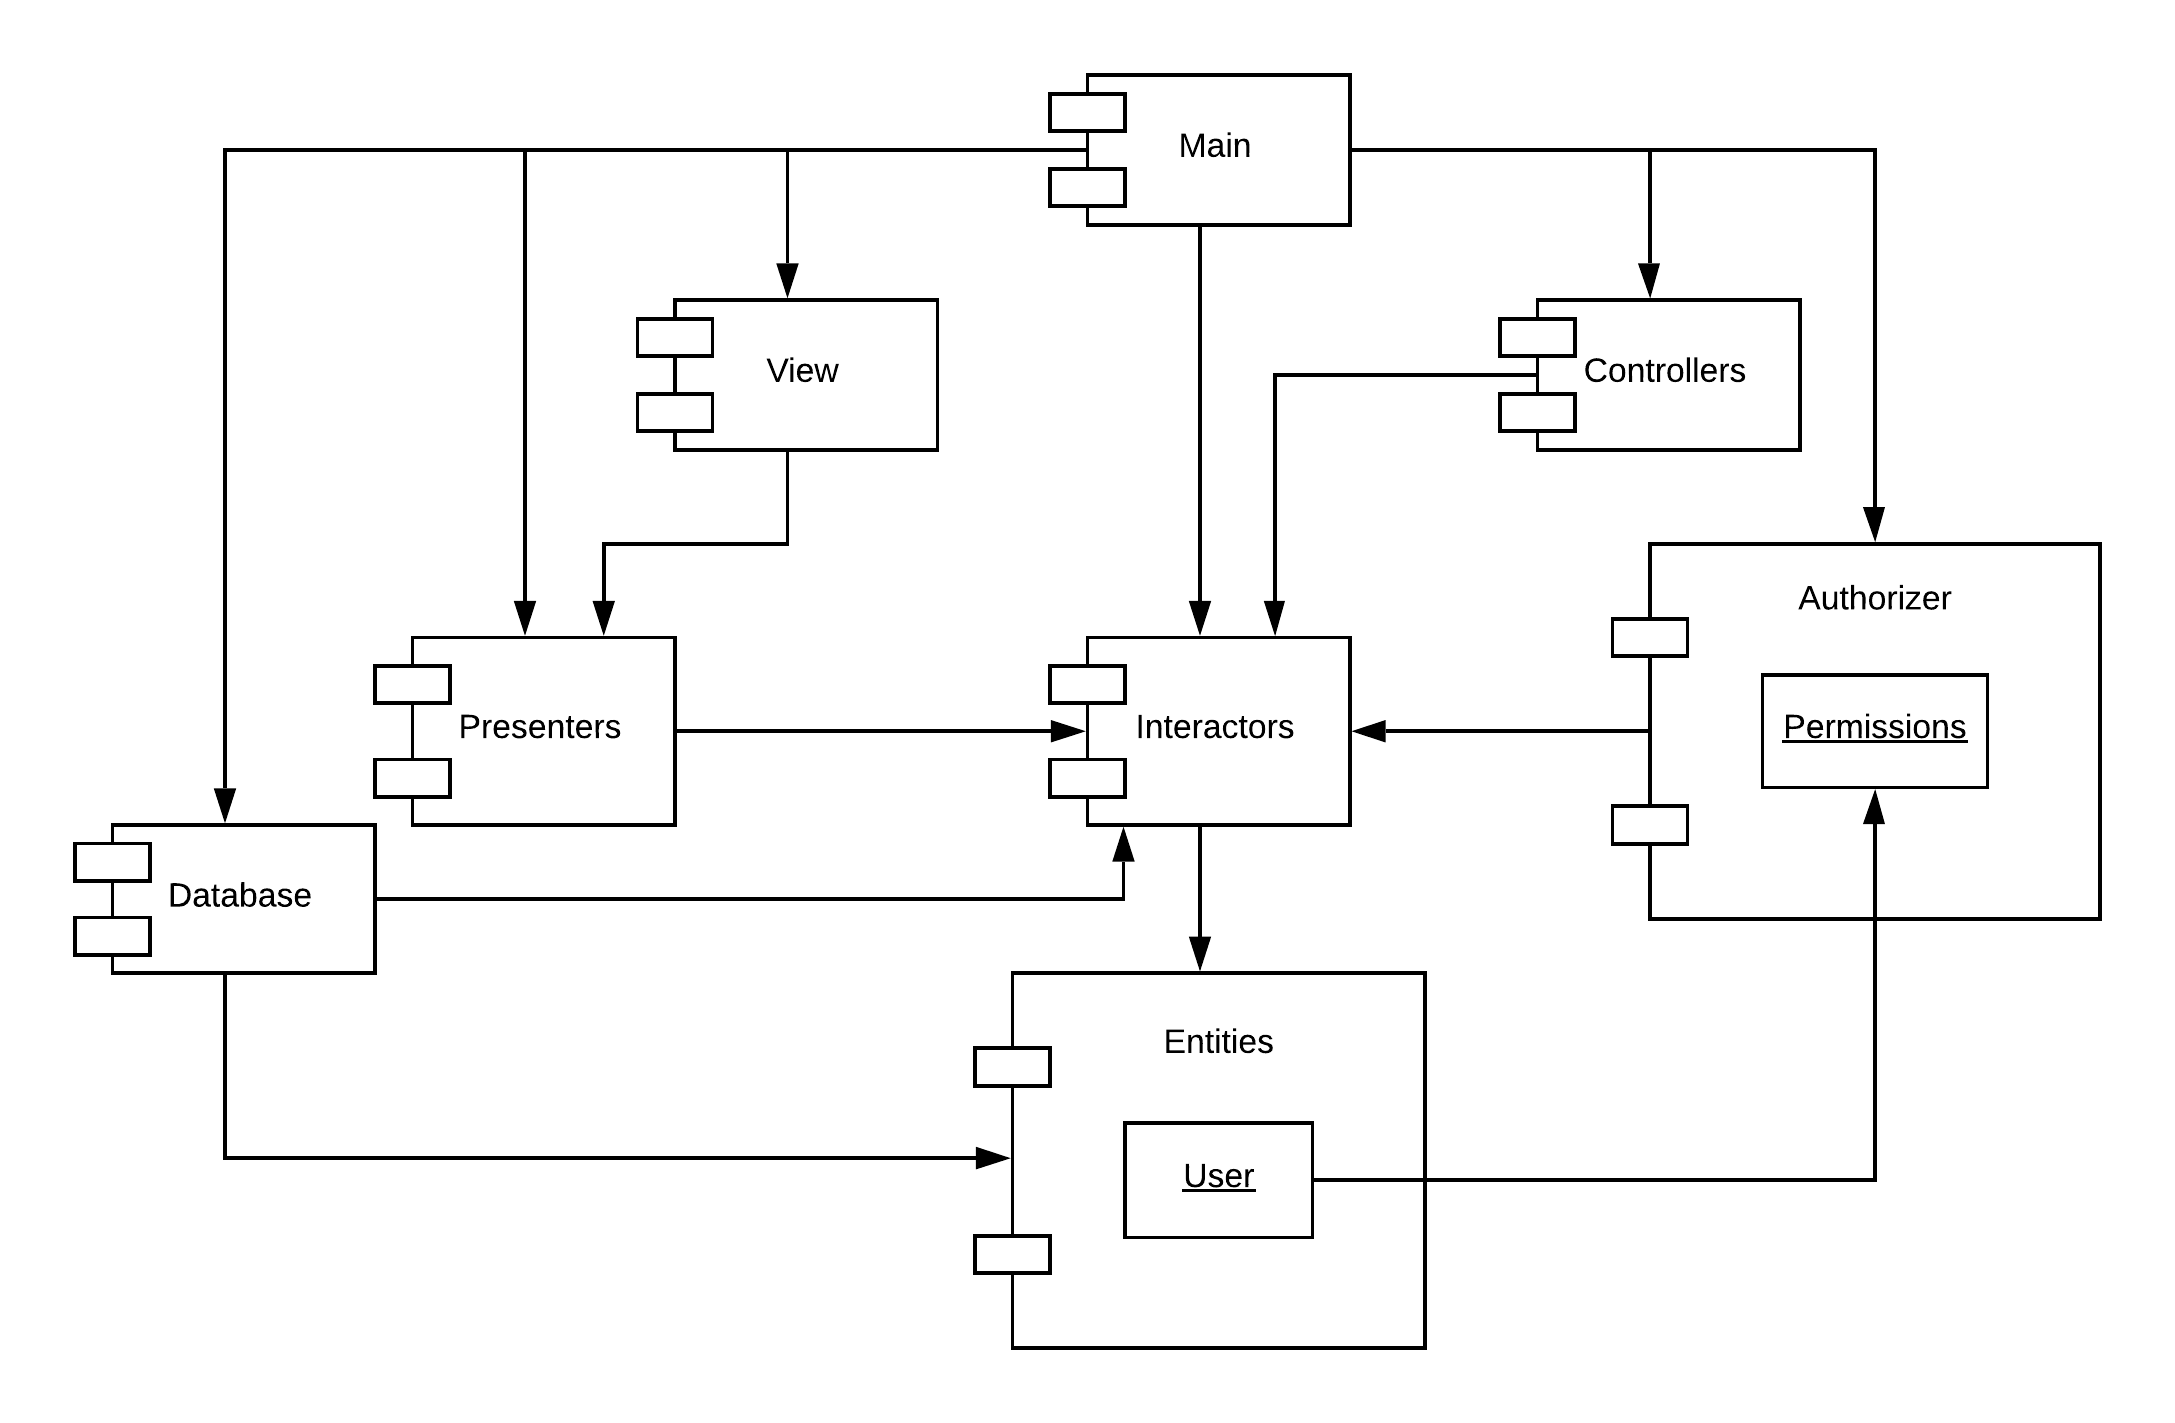
\includegraphics[width=1\textwidth]{images/adp.png}
 	\caption{Ein Abh�ngigkeitszyklus(basierend auf \cite{CA:18}, S.134 Abb. 14.2. sowie S.135, Abb.14.3)}
 	\label{fig:adp}
 \end{figure}
 
 
 \begin{figure}[htbp] 
 	\centering
 	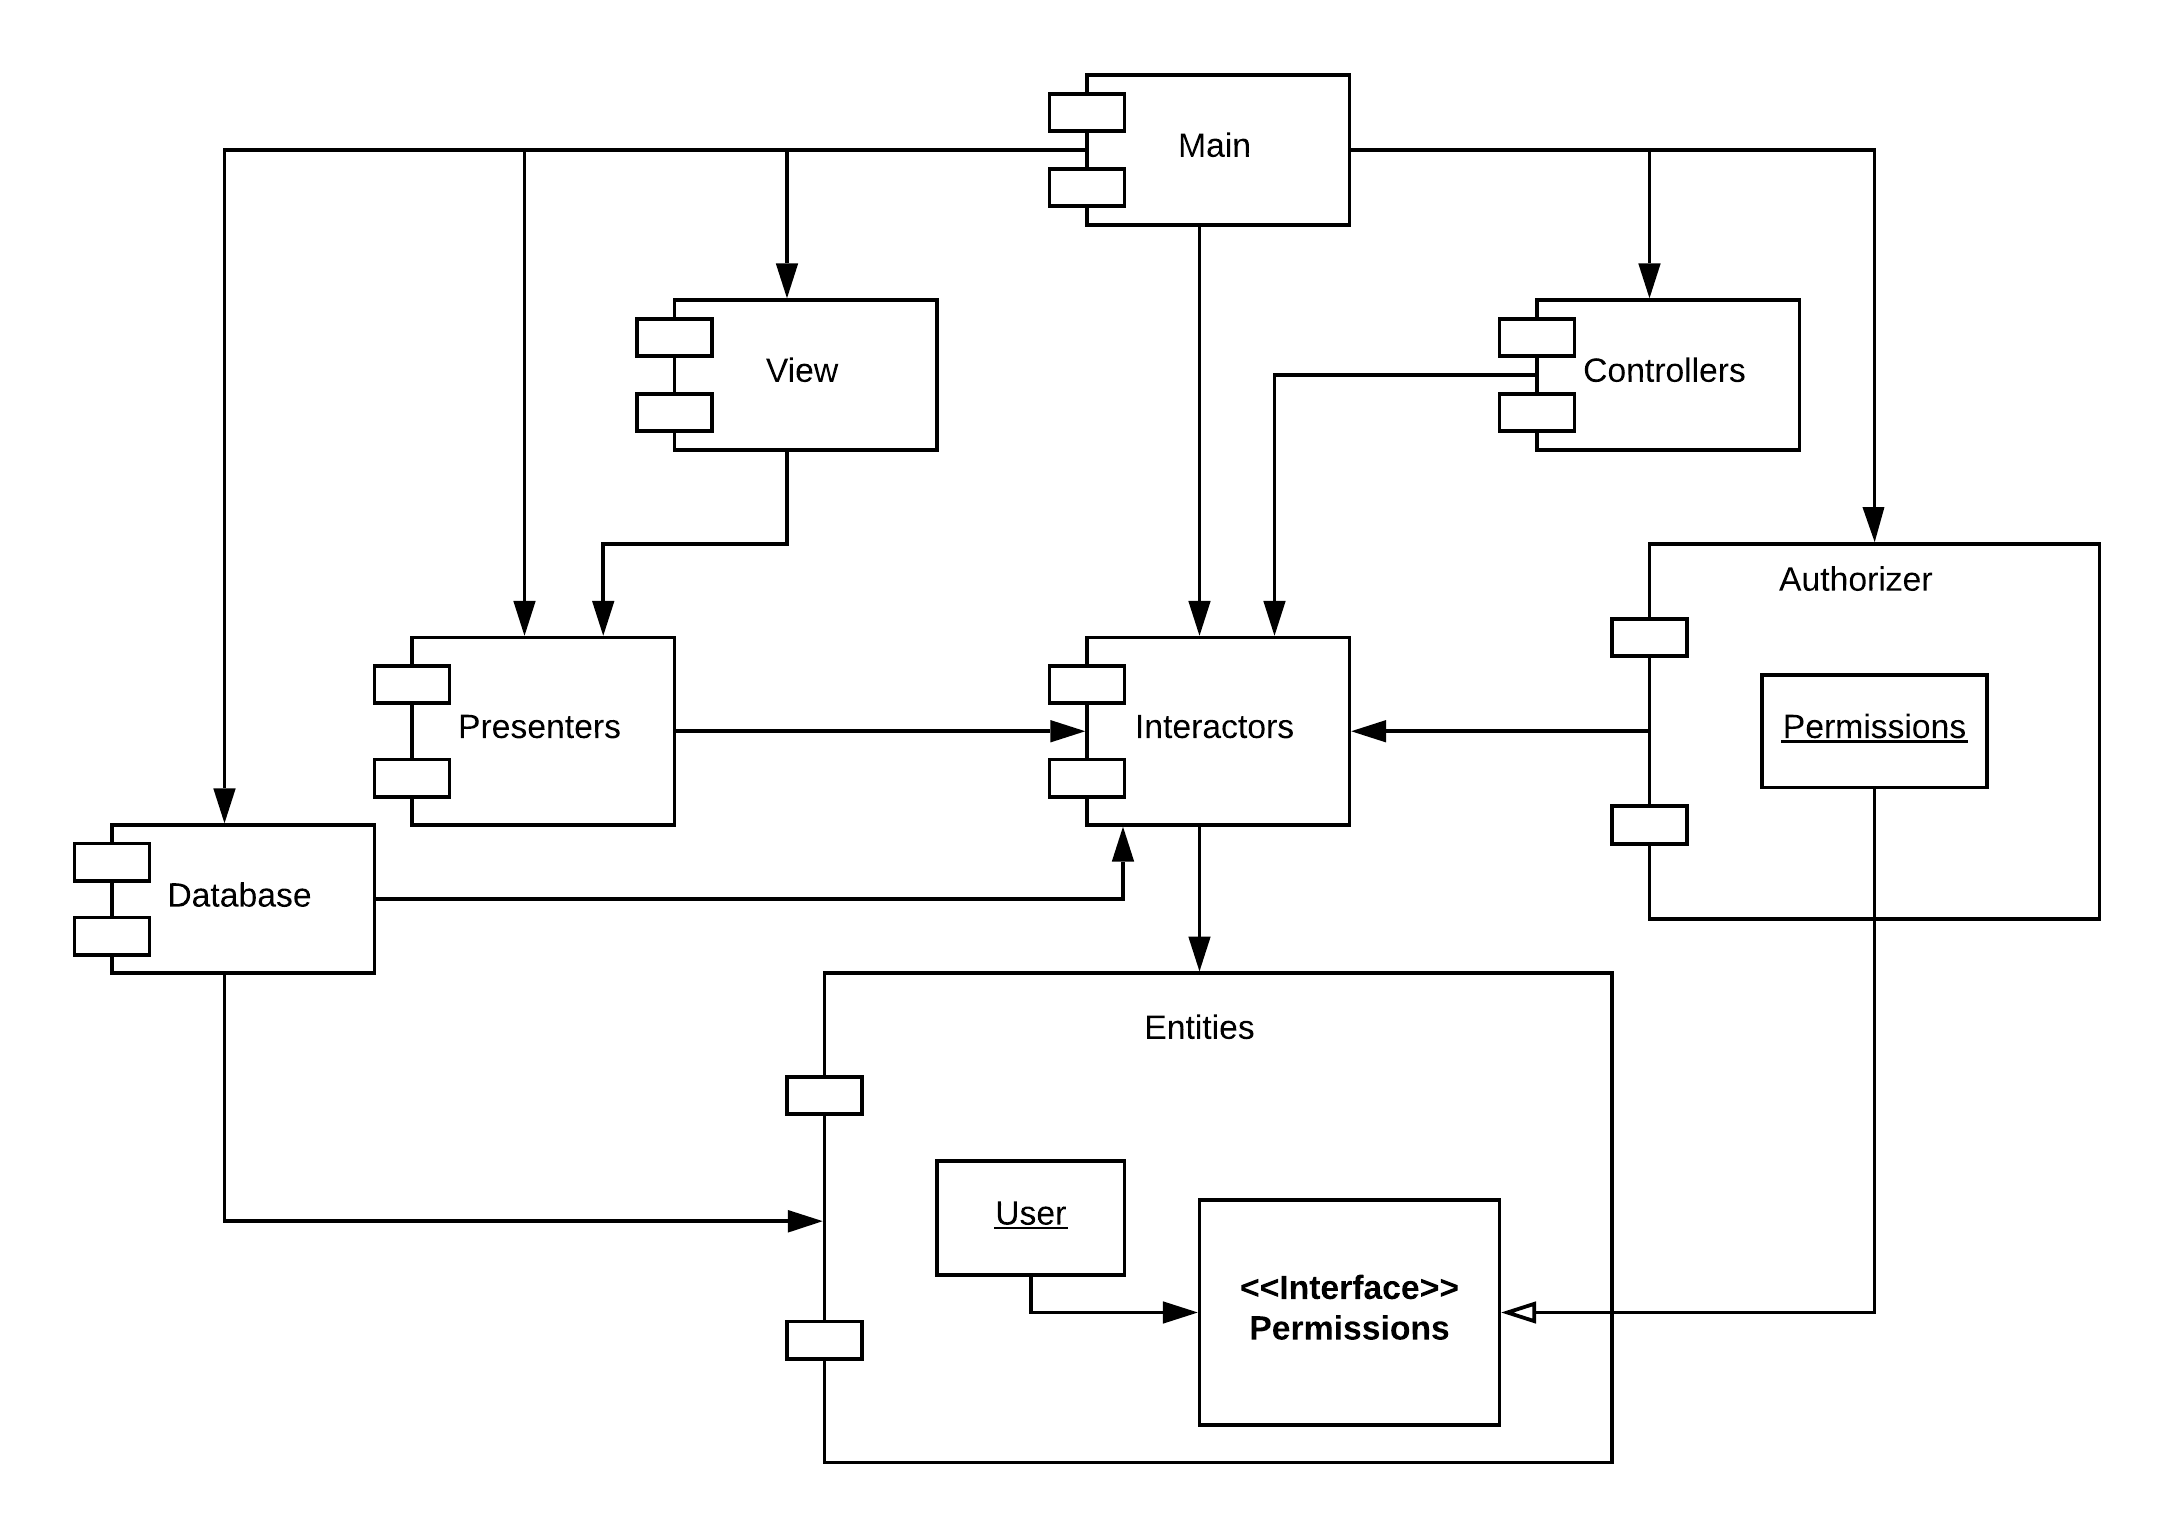
\includegraphics[width=1\textwidth]{images/adp_2.png}
 	\caption{Aufl�sung des Abh�ngigkeitszyklus mittels DIP (basierend auf \cite{CA:18}, S.134 Abb. 14.2. sowie S.135, Abb.14.3)}
 	\label{fig:loes1_adp}
 \end{figure}
 
 
 

%\subsubsection{Das Reuse-Release-Equivalence-Prinzip (REP)}
%\subsubsection{Das Common-Closure-Prinzip (CCP)}
%\subsubsection{Das Common-Reuse Prinzip (CRP)}




\subsubsection{Das Stable-Dependencies-Prinzip (SDP)}
Das Stable-Dependencies-Prinzip bezieht sich auf die Komponentenkopplung  und lautet: \glqq Abh�ngigkeiten sollten in dieselbe Richtung verlaufen wie sie Stabilit�t.\grqq (\cite{CA:18}, S.137, Z.16). \\
Demnach sollen stabile Komponenten nicht von instabilen Komponenten abh�ngen, die sich mit hoher Wahrscheinlichkeit �ndern werden.
Stabile Komponenten lassen sich nur schwer modifizieren und behindern damit die �nderungen an der instabilen Komponente, da sie nur schwer daran angepasst werden k�nnen. Stattdessen sollen die instabilen von den stabilen Komponenten abh�ngen\cite{CA:18}, S.137).\\
Stabilit�t im Zusammenhang mit Software gibt an, wie viel Aufwand erforderlich ist, eine Komponente zu �ndern. Je gr��er der Aufwand, desto stabiler ist sie. Eine Komponente ist sehr stabil, wenn sie viele eingehende , aber kaum ausgehende Abh�ngigkeiten aufweist (\cite{CA:18}, S. 138). Die Instabilit�t einer Komponente $I \in [0,1]$ l�sst sich wie in Formel \ref{eq} angegeben bestimmen (\cite{CA:18}, S.139), wobei 0 maximal stabil entspricht und $\#$ ist die Anzahl bezeichnet. Verst��e gegen das SDP lassen sich mit dem DIP (siehe \ref{dip}) l�sen (\cite{CA:18}, S.139-142).


\begin{equation}
\label{eq}
	I=\frac{\# Ausgehende Abh\ddot{a}ngigkeiten}{\# Eingehende Abh\ddot{a}ngigkeiten +  \# Ausgehende Abh\ddot{a}ngigkeiten}
\end{equation}



\subsubsection{Das Stable-Abstractions-Prinzip (SAP)}
Das Stable-Abstractions-Prinzip bezieht sich ebenfalls auf die Komponentenkopplung und lautet:
\glqq Eine Komponente sollte ebenso abstrakt sein, wie sie stabil ist.\grqq (\cite{CA:18}, S.143, Z.14). \\
Damit sollen stabile Komponenten aus Schnittstellen sowie abstrakten Klassen und instabile Komponenten aus konkreten Klassen bestehen. Diese Abstraktion erlaubt es, stabile Komponenten trotz ihrer Stabilit�t erweitern zu k�nnen.\\
SAP und SDP zusammengenommen ergeben das DIP auf Komponentenebene. Der wesentliche Unterschied ist, dass Komponenten im Gegensatz zu Modulen nicht entweder abstrakt oder konkret sind, sondern sich auch dazwischen befinden k�nnen.
Der Grad der Abstraktion einer Komponente $A \in [0.1]$ l�sst sich genau wie Stabilit�t als Software-Metrik messen mittels der in \ref{eq2} angegebenen Formel (\cite{CA:18}, S.144), wobei 1 f�r maximal abstrakt steht.
\begin{equation}
\label{eq2}
A=\frac{\# abstrakte Klassen/Schnittstellen}{\# Gesamtzahl Klassen}
\end{equation}



\section{Design-Patterns}
Es exisitiert eine breite Auswahl von Abstrahierungs- und Genreralisierungs-Design-Patterns, die �nderungen vereinfachen. Im Folgenden werden Beispiele aufgef�hrt.


\subsection{Abstract Factory}
Das DIP (siehe Abschnitt \ref{dip} bedingt, dass konkrete, fl�chtige Objekte nicht ohne Weiteres erzeugt werden k�nnen, denn jede Objekterzeugung stellt eine Abh�ngigkeit zu einer konkreten Klasse des Objektes dar (\cite{CA:18}, S.109). 
Abhilfe schafft das Design-Pattern Abstract Factory. Dieses Pattern erlaubt es, Familien verwandter Objekte zu erzeugen, ohne deren konkrete Klassen zu spezifizieren, d.h. ohne Abh�ngigkeiten zu jenen Objekten herzustellen (\cite{pat}, S.90). \\
In Abbildung \ref{fig:fact} ist das Pattern am Beispiel einer plattform�bergreifenden grafischen Anwendung gezeigt. In der Mitte befindet sich das Interface GUIFactory, dies ist die Abstract Factory. Hier werden Methoden f�r die konkreten Factories vorgegeben. Windows Factory und MacFactory sind die konkreten Factories, sie implementieren die Methoden der Abstract Factory. Das Interface Checkbox stellt ein abstraktes Produkt dar, das von den konkreten Produkten WindowsCheckbox und MacCheckbox implementiert wird, analog verh�lt es sich mit dem Interface Button (\cite{pat}, S.96). \\
Der erste Vorteil besteht in der Konsistenz der Produkte: Die WindowsFactory stellt nur zueinander passende Windows UI-Elemente her, analog bei der MacFactory. Das Pattern l�sst sich um eine Linux-Factory erweitern, die konsistente Linux UI-Elemente enth�lt. \\
Der zweite Vorteil besteht darin, dass die Anwendung lediglich von GUIFactory abh�ngig ist, d.h. von einer Abstraktion, was dem DIP entspricht. \\
Es stellt sich die Frage, an welcher Stelle eine Factory-Instanz erzeugt wird, z.B. eine WindowsFactory. Dies geschieht  in einer konkreten Klasse innerhalb einer konkreten Komponente, wie etwa in der main-Methode, wobei die erzeugte Instantz in einer globalen Variablen gespeichert wird, auf welche die Anwendung dann global zugreifen kann (\cite{CA:18}, S.110).


 \begin{figure}[htbp] 
	\centering
	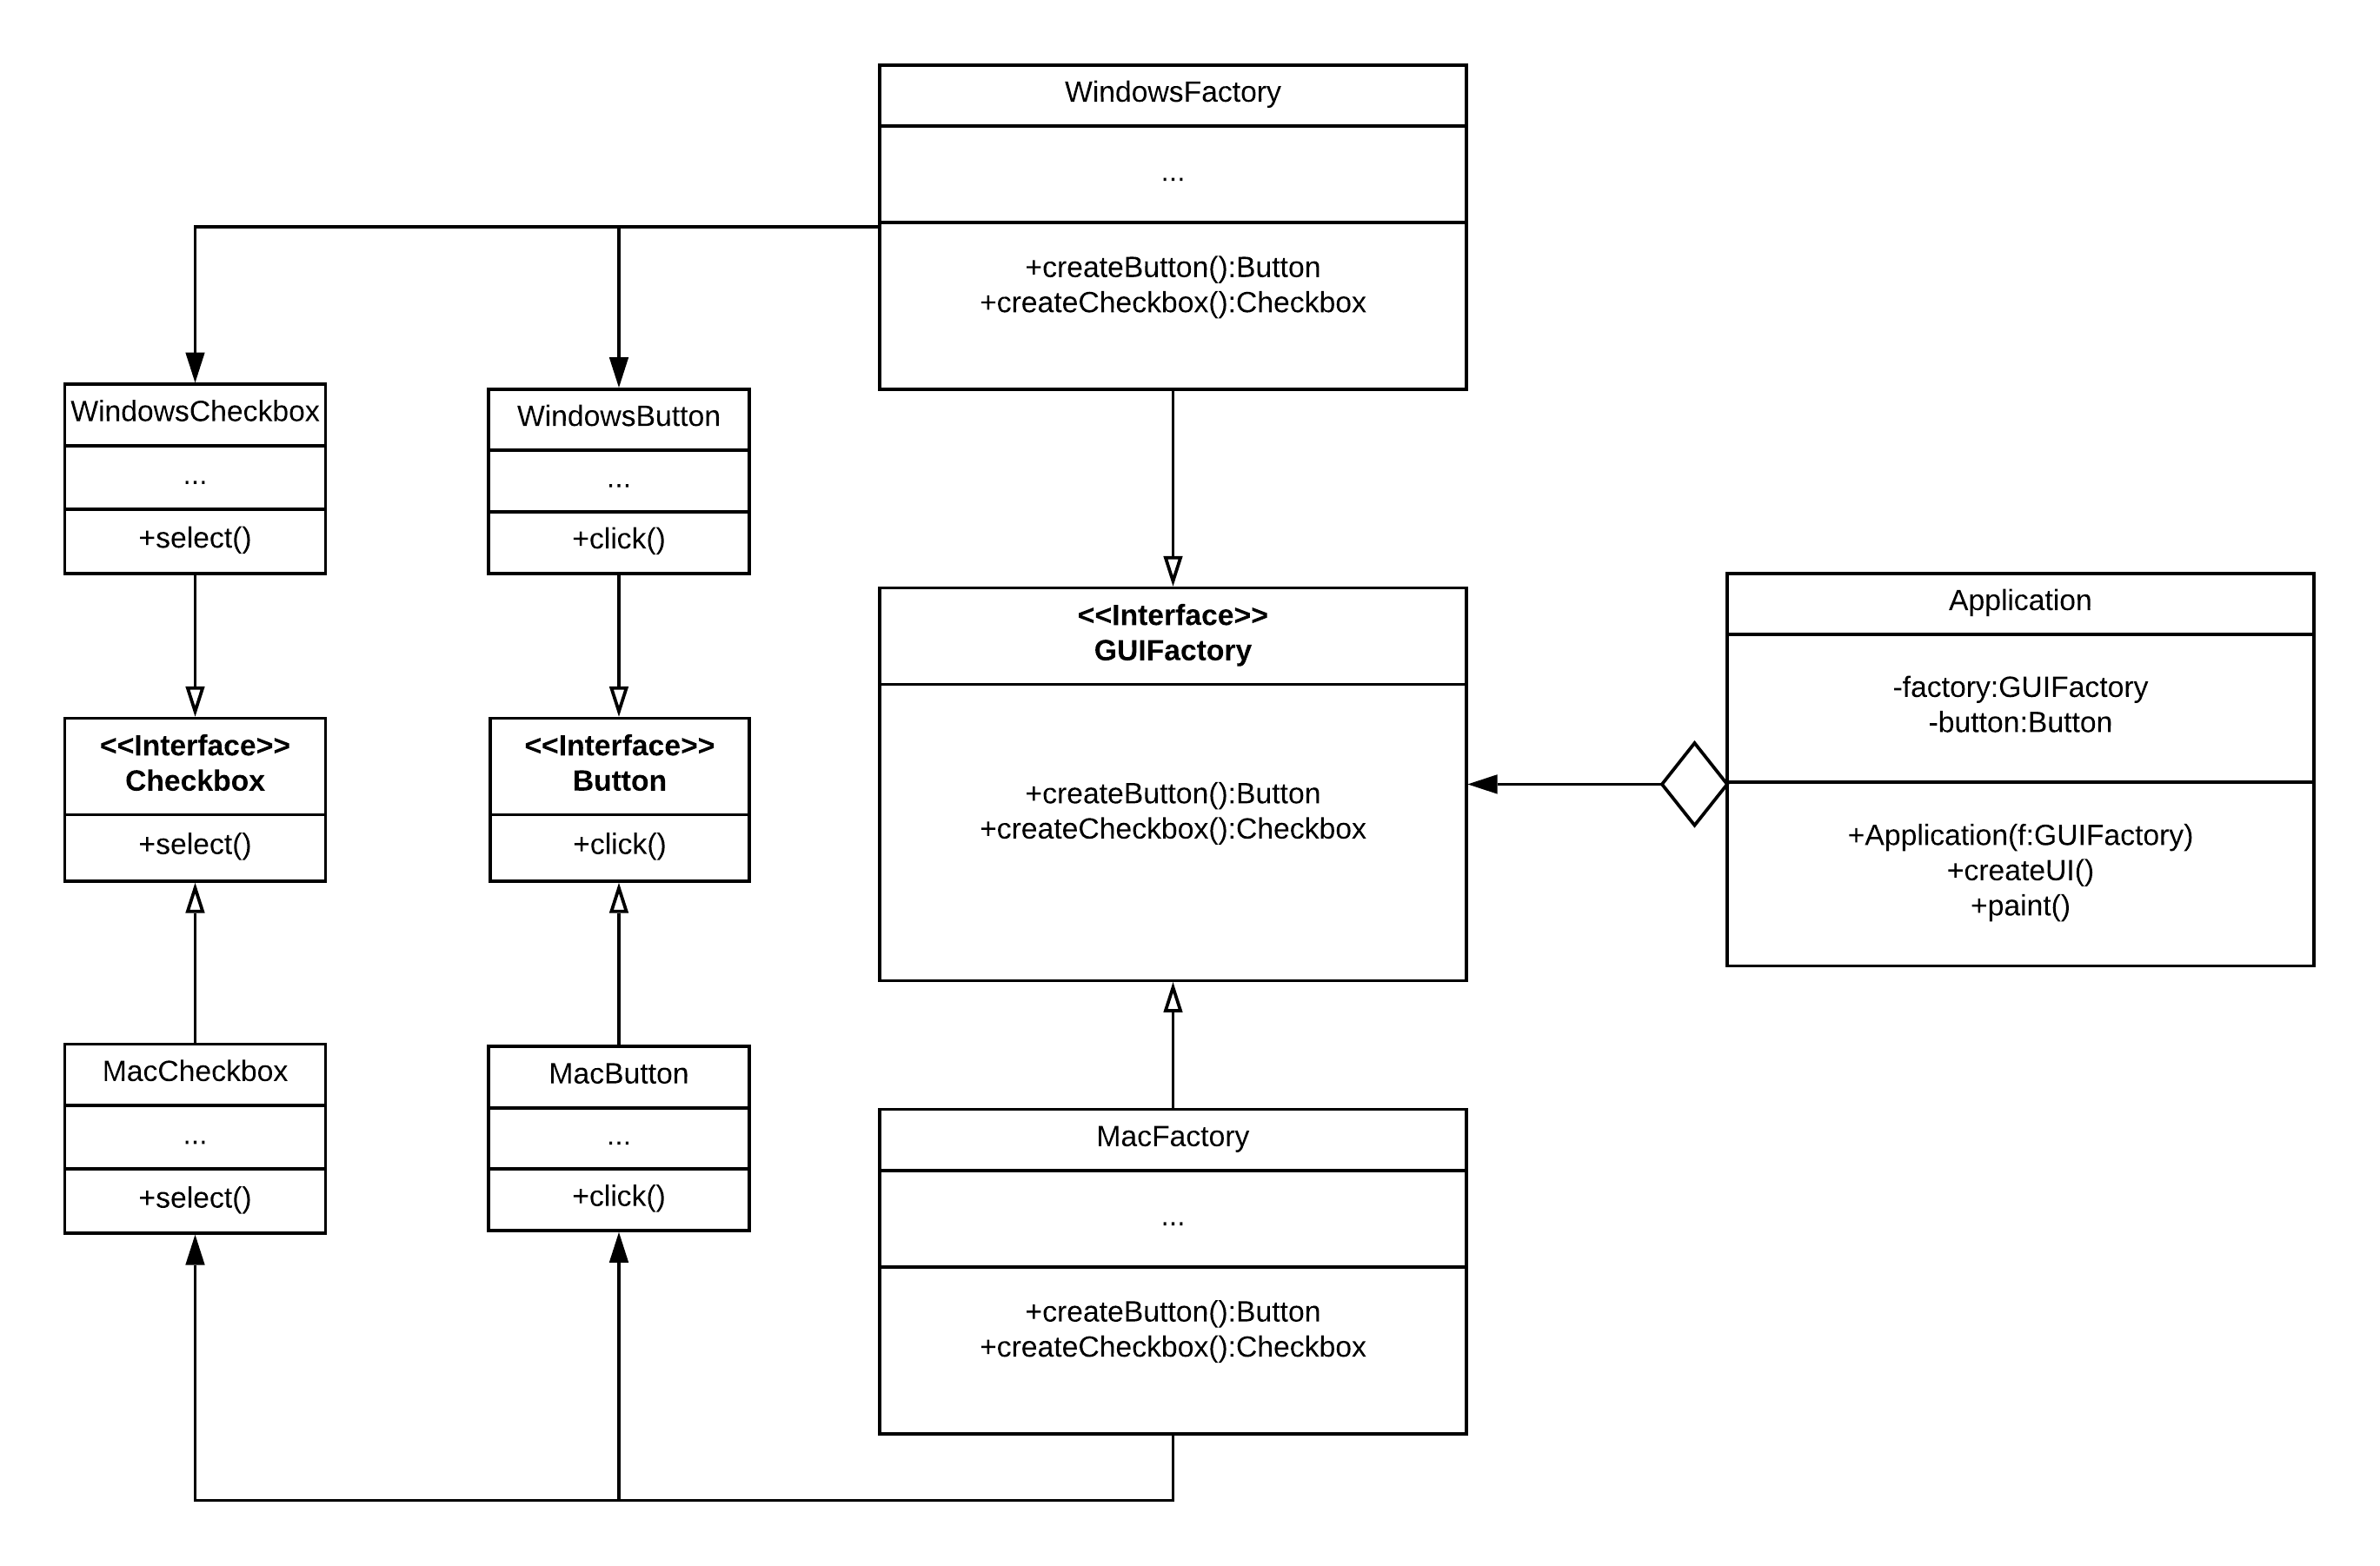
\includegraphics[width=1\textwidth]{images/abstract_factory.png}
	\caption{Design Pattern Abstract Factory (Abbildung basierend auf \cite{pat}, S.97)}
	\label{fig:fact}
\end{figure}


\subsection{Dependency Injection}
Dieses Design-Pattern hilft, �bergeordnete Module vor den Implementierungsdetails von untergeordneten Modulen zu sch�tzen (\cite{SSA:12}, S.555). \\
Abbildung \ref{fig:dep_inj} zeigt Constructor Dependency Injection an einem konkreten Beispiel. Die Klasse \textit{PaymentTerms} beinhaltet alle Informationen, die zur Berechnung der monatlichen Kosten eines Kredits notwendig sind. Die Klasse \textit{PaymentCalculator} enth�lt die Methode \textit{getMonthlyPayment()}, d.h. hier wird die konkrete Berechnung durchgef�hrt. Das Problem besteht darin, dass \textit{PaymentTerms} diese Methode aufrufen muss und ohne Dependency Injection direkt von \textit{PaymentCalculator} abh�ngig w�re. Dies w�re bedenklich: Es k�nnnten neue Arten von \textit{Calculator}-Klassen hinzukommen, welche die Berechnung anders durchf�hren, oder vielleicht gibt es auch bereits mehrere solcher \textit{Calculator}-Klassen. Dann sollte es nicht in der Klasse\textit{ PaymentTerms} entschieden werden, welche Berechnung verwendet wird, sondern in einem �bergeordneten Modul. \\
Constructor Dependency Injection l�st dies folgenderma�en: Es wird ein Interface erzeugt, hier \textit{IPaymentCalculator} genannt, das die ben�tigte Methode enth�lt und das von \textit{PaymentCalculator }und allen m�glichen weiteren \textit{Calculator}-Klassen implementiert wird. Der Klasse \textit{PaymentTerms} wird im Konstruktor ein\textit{ IPaymentCalculator}-Objekt �bergeben. Damit besteht nur noch eine Abh�ngigkeit zu einer Abstraktion, was dem DIP entspricht (siehe \ref{dip}). Der konrkete Calculator-Typ wird erst zur Laufzeit entschieden, da die Abh�ngigkeit �ber den Konstruktor injected wird, was den Namen des Patterns erkl�rt. Das bietet eine hohe Flexibilit�t, denn die Implementierungsdetails in \textit{PaymentTerms} stellen nun kein Problem mehr da. Wird ein anderer Berechnungstyp ben�tigt, kann von einem �bergeordneten Modul aus einfach ein anderes \textit{IPaymentCalculator}-Objekt �bergeben werden. Es ist anzumerken, dass Constructor Injection nur ein m�glicher Typ von Dependency Injection ist. Es existieren zudem noch Setter Injection und Interface Injection \cite{dep}. Dependency Injection ist auch unter dem Namen Inversion of Control bekannt (\cite{SSA:12}, S.555).


 \begin{figure}[htbp] 
	\centering
	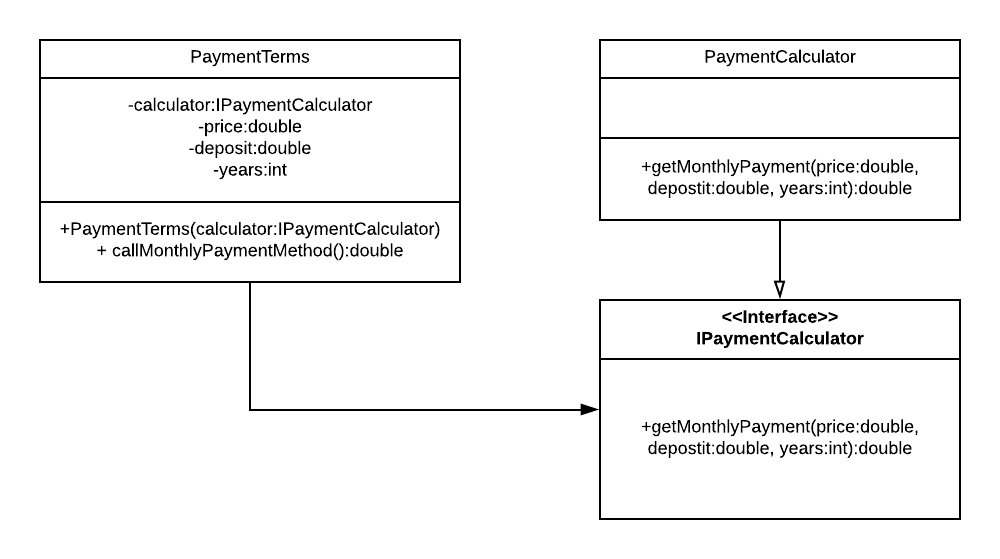
\includegraphics[width=1\textwidth]{images/dep_inj.png}
	\caption{Constructor Dependency Injection (Abbildung basierend auf \cite{dep})}
	\label{fig:dep_inj}
\end{figure}



\subsection{Weitere Patterns}
Weiter Patterns, die �nderungen vereinfachen, sind das Prototype Pattern (\cite{pat} S.124), das direkte Abh�ngigkeiten beim Kopieren von Objekten vermeidet, sowie das Adapter Pattern, dass es Objekten mit inkompatiblen Schnittstellen erlaubt, dennoch zusammenzuarbeiten (\cite{pat}, S.150).


\section{Erweiterbare Interfaces}
Diese Architekturtaktik bezieht sich auf die Gestaltung von Interfaces. Ihnen sollte besondere Aufmerksamkeit zukommen, denn �nderungen an Interfaces haben den gr��ten Einfluss auf das Systen und verursachen damit die gr��ten Kosten. Wird beispielsweise ein Parameter einer Funktion ge�ndert, m�ssen alle Klassen angepasst werden, welche das Interface implementieren und damit diese Funktion verwenden. \\
Eine m�gliche L�sung besteht darin, anstatt vieler Paramter Objekte oder andere strukturierte Datentypen, z.B. structs in C++, in der Funktion zu �bergeben. Alle Parameter sind dann als Attribute in der Klasse des Objekts vorhanden. Der Vorteil ist, dass Attribute sich optional gestalten lassen, indem sie mit Default-Werten initialsiert werden.\\
Analog verh�lt es sich mit Information Interfaces. Anstelle von Objekten k�nnen selbstbeschreibende Nachrichtenformate �bergeben werden, wie z.B. XML. Wenn das Nachrichtenformat es zul�sst, wie XML, k�nnen Elemente optional gesetzt werden. \\
Eine solch flexible Gestaltung von Interfaces geht zulasten von Verst�ndlichkeit und Testbarkeit, da es beispielsweise nur schwer auff�llt, wenn Elemente fehlen. Es kann zudem auch zu Performanzeinbu�en kommen. Darum gilt es abzuw�gen, welche Interfaces in Zukunft wahrscheinlich erweitert werden und eine solche Flexibilit�t ben�tigen (\cite{SSA:12}, S.553-554). 


\section{Metamodell-basierte Architekturstile}
Metamodell-basierte Architekturstile sind, wie der Name bereits sagt, eigene Architekturstile, d.h. es handelt sich hierbei um eine sehr tiefgreifende Architekturtaktik. Metamodell-basierte Systeme sind von Grund auf auf �nderungen eingestellt und ausgelegt (\cite{SSA:12}, S.555). Man bezeichnet sie auch als Metasysteme, da es sich um Systeme von Systemen handelt (\cite{meta}, S.1). \\
Metamodell-basierten Architekturstilen gemeinsam ist ein �bergeordnetes Metamodell, welches das Zusammenspiel der Komponenten koordiniert. Die Konfigurationen des Metamodells entscheiden, wie die Komponenten zur Laufzeit zusammengesetzt werden. Oft reicht es, bei �nderungen nur die Konfigurationen des Metamodells anzupassen. Da die Konfigurationen jedoch zur Laufzeit eingelesen und umgesetzt werden, sind Metasysteme im Hinblick auf Performanz eingeschr�nkt. Der hohe Grad an Flexibilit�t schl�gt sich zudem auch in einer erh�hten Komplexit�t nieder, die sowohl das Entwickeln als auch das Testen erschwert (\cite{SSA:12}, S.556).\\
Es gibt verschiedene Arten von Metasystemen. Diese n�her zu erl�utern, w�rde den Rahmen der Ausarbeitung sprengen. Es sei an dieser Stelle jedoch ein Beispiel genannt. \\
Nach \cite{meta} ist ein Metasystem ein gro� angelegtes, verteiltes System, dessen Komponenten Enterprise-Systeme sind, die durch den Governance Mechanismus des Metamodells miteinander verkn�pft sind, um ein gemeinsames strategisches Ziel zu erreichen (\cite{meta}, S.1, Z.66-73). Das �bergeordnete Governance System leitet, �berwacht und koordiniert alle Operationen des Metasystems. Die untergeordneten Enterprise-Systeme, d.h. die Komponenten des Systems, k�nnen bei Bedarf rekonfiguriert werden, ohne dass die Implementierung des Systems angepasst werden muss. Zudem lassen sich die Enterprise-Systeme austauschen, es lassen sich zudem Systeme entfernen und neue hinzuf�gen. Damit ist diese Architektur hochflexibel und passt sich einer sich �ndernden Umgebung in co-evolution�rer Weise an (\cite{meta}, S.2). Anwendung findet ein solcher Architekturstil beispielsweise bei gro�en Energieverteilungs-, Informations- oder Kommunikationsnetzwerken oder auch bei Netzwerken, welche die Luftfahrt kontrollieren. Dort m�ssen die Systeme sich an st�ndig �ndernde Informationen und Bedingungen anpassen. Nachteil ist hierbei, wie bei allen Metamodell-basierten Systemen, eine hohe Komplexit�t (\cite{meta}, S.1). \\
Nicht alle Metasysteme sind gleich so komplex, dass sie sich aus mehreren Enterprise-Systemen zusammensetzen. Das Beispiel soll jedoch veranschaulichen, dass Kosten und Nutzen beim Einsatz eines solchen Stils abgew�gt werden m�ssen. Nur, wenn wirklich ein solch hoher Grad an Flexibil�t ben�tigt wird, sollten Metamodelle zum Einsatz kommen. 






\section{Variation Points}
Diese Architekturtaktik besteht darin, Variation Points zu verwenden. \\
Dies sind lokale Design-L�sungen, um bestimmte �nderungen an bestimmten Stellen im System zu unterst�tzen. Hierbei m�ssen die Stellen, an denen Variation Points erforderlich sind, identifiziert werden. (\cite{SSA:12}, S.556). \\
Im ersten Abschnitt werden allgemeine Vorgehensweisen pr�sentiert, worauf im zweiten konkrete Design-Patterns folgen, mit denen sich Variability realsieren l�sst. 

\subsection{Vorgehensweisen} 
Ein m�gliches Vorgehen besteht darin, Elemente austauchbar zu gestalten.
Werden die SOLID-Prinzipien konsequent befolgt, ist dies kein Problem. Im Idealfall sind Implementierung und Interface getrennt und die Implementierung h�ngt vom Interface ab. Dann kann die Implementierung des Interfaces durch eine andere Implementierung des Interfaces ausgetauscht werden. Dies entspricht sowohl dem DIP (siehe \ref{dip}) als auch dem LSP (siehe \ref{lsp}). \\
Eine weitere Vorgehensweise besteht darin, Konfigurationen zu verwenden.
Bestimmte Teile des Systemverhaltens lassen sich durch Parametrisierung steuern. Dann lassen sich �nderungen oft alleine durch das Anpassen der Parameter realisieren. . \\
Variation Points k�nnen au�erdem erreicht werden, indem selbstbeschreibende Daten sowie eine generische Verarbeitungsweise gew�hlt werden.
Bei solchen selbstbeschreibenden Datenformaten wie z.B. XML lassen sich die Informationen nutzen, um die Daten generisch zu verarbeiten. \\
Au�erdem ist es von Vorteil, die Verarbeitung des Datenformats von der logischen Verarbeitung getrennt zu halten. Dann l�sst sich das Datenformat wesentlich einfacher �ndern, wie z.B. beim Umstieg von CSV zu XML. \\
Zudem sollten gr��ere Prozesse stets in Teilschritte unterteilt werden. Dies bietet den Vorteil, dass einzelne Schritte austauschbar sind (\cite{SSA:12}, S.556-557).


\subsection{Beispiele}
In diesem Abschnitt werden Design-Patterns vorgestellt, die Variability erm�glichen. 

\subsubsection{Facade}
Dieses Pattern bietet Variability bei der Verwendung von Biblithoken, Frameworks oder einer anderen komplexen Menge an Klassen, indem 
es eine vereinfachte Schnittstelle zu jenen Elementen zur Verf�gung stellt (\cite{pat}, S.210). Diese Schnittstelle enth�lt nur die Methoden, die wirklich ben�tigt werden. Damit ist das System nicht mehr so stark an die externe Bibliothek, das Framework etc. gekoppelt und �nderungen daran, die zu erwarten sind, wirken sich weniger stark aus (\cite{pat}, S.211). Upgrades zu neueren Versionen oder das Austauschen der Software hinter der Schnittstelle stellen mit diesem Design-Pattern kein Problem mehr dar (\cite{pat}, S.214). 

\subsubsection{Template Method}
Dieses Design Pattern bietet Variation Points innerhalb eines Algorithmus. Das Template Method Pattern definiert das Grundger�st eines Algorithmus in der Superklasse und l�sst Subklassen bestimmte Schritte des Algorithmus �berschreiben, ohne dabei die Struktur des Algorithmus zu ver�ndern. Die Verwendung bietet sich dann an, wenn der Algorithmus zwar grundlegend gleich bleibt, aber Details stellenweise angepasst werden m�ssen. 
Beispielsweise ist in einer Data-Mining-Anwendung Variabilit�t bez�glich des Datenformats erforderlich. Der Algorithmus sollte nicht jedes Mal neu geschrieben werden m�ssen, wenn auf ein anderes Datenformat, z.B. von CSF auf PDF, umgestiegen wird.
 Der Algortihmus wird hierzu in einzelne Methoden unterteilt, wobei jede Methode einen Schritt darstellt. Die Abfolge dieser Methoden wird in eine einzige �bergreifende Template Method geschrieben, die entweder abstrakt ist oder eine Default-Implementierung aufweist. Die Subklasse implementiert dann alle abstrakten Schritte und �berschreibt bestimmte Methoden, wenn dies ben�tigt wird (\cite{pat}, S.381-383).



%\subsubsection{Chain of Responsibility}

%\subsubsection{Template Method}
%\subsubsection{Visitor}
%objectifier pattern
%Template and hook
%Template class https://refactoring.guru/design-patterns/template-method
% Dimensional Class Hierarchies
% Bridge https://refactoring.guru/design-patterns/bridge
% Visitor https://refactoring.guru/design-patterns/visitor
% Facet Classifications
 
\subsubsection{Weitere Patterns}
 Weitere Patterns, die Variability erlauben, sind Bridge (\cite{pat}, S.163-177), Chain of Responsibility (\cite{pat}, S.250-267) sowie das Visitor Pattern (\cite{pat}, S.393-408).


\section{Extension Points}
Diese Architekturtaktik besteht darin, Extension Points zu nutzen.
Extension Points sind Schnittstellen f�r Erweiterungen (\cite{extension}, S.1). Sie geben vor, an welchen Stellen des Systems Erweiterungen ankn�pfen sollen und welche Voraussetzung diese Erweiterungen erf�llen m�ssen. \\
Hinter Extension Points steht ein Extension Mechanismus, d.h. die Art und Weise wie die Erweiterung intern vom System unterst�tzt und umgesetzt wird, inklusive Ber�cksichtigung der Software-Umgebung (\cite{extension}, S.1). \\
Bei vielen Standardsoftwares werde Extension Points mitgeliefert, sodass an diese angekn�pft werden kann. So unterst�tzt die J2EE Plattform beispielsweise die Anbindung neuer Datenbanktypen und externer Systeme(\cite{SSA:12}, S.558). Ein anderes Beispiel f�r Standardsoftware, die Extension Points anbietet, stellt Eclipse dar \cite{extension}. Plug-Ins k�nnen an diese Extension Points ankn�pfen (\cite{eclipse}).\\
Die Vorteile bestehen darin, dass den Entwicklern bei der Erweiterung eine Menge Arbeit abgenommen wird. Zudem ist klar, wo erweitert werden muss und wie. Dennoch sollten Extension Points nicht blind genutzt werden, denn schlecht umgesetzte Extension Mechanisms k�nnen Performanzeinbu�en und erh�hte Komplexit�t mit sich bringen (\cite{extension}, S.6). \\
Es sei zudem angemerkt, dass es ggf. sinnvoll sein kann, selbst Extension Points in das System enzubauen, wenn klar ist, dass andere Entwickler in Zukunft das System erweitern werden.




\section{Reliable Change}
Bei dieser Architekturtaktik \textit{reliable change} geht es darum, �nderung so zuverl�ssig und sicher wie m�glich umzusetzen (\cite{SSA:12}, S.558). Es gibt einige Ma�nahmen, um dies zu erreichen. \\

\subsection{Konfigurationsmanagement}
An erster Stelle ist hier das Konfigurationsmanagement zu nennen. Konfigurationsmangament fasst alle Aktivit�ten zusammen, die zur Verwaltung der Konfigurationen dienen (\cite{SWT:12}, S.253, Z.29-30). Eine Konfiguration ist \glqq die Anordnung eines Computersystems bzw. einer Komponente oder eines Systems, wie sie durch Anzahl, Beschaffenheit und Verbindung seiner Bestandteile definiert ist \grqq (\cite{SWT:12}, S.253, Z.24-26). F�r Konfigurationsmanagement exisiteren zahlreiche Tools, die eingesetzt werden k�nnen. Konfigurationsmanagement schlie�t Versionskontrolle mit ein (\cite{SWT:12}, S.205).

\subsection{Automatisieren}
Vorg�nge wie der Build-Prozess, der Release-Prozess und das Testen sollten automatisiert werden. So werden die Prozesse zuverl�ssig, konsistent und lassen sich wiederholen mit demselben Ergebnis. \\
Automatisiertes Testen sollte auf keinen Fall vernachl�ssigt werden, denn es ist wichtig, sicherzustellen, dass sich mit den �nderungen keine Fehler eingeschlichen haben. Daf�r m�ssen hunderte bis tausende Tests durchgef�hrt werden, was sich manuell nicht mit vertretbarem Aufwand erreichen l�sst (\cite{SSA:12}, S.559). Auch f�r das Automatisierte Testen existieren zahlreiche Tools.
\subsection{Dependency Analysis}
Eine Depency Analysis l�sst sich mit Tools durchf�hren und gibt hilfreichen Aufschluss �ber unentdeckte Abh�ngigkeiten, die sonst eventuell �bersehen worden w�ren. Anhand von Dependency Analysis lassen sich die Auswirkungen von �nderungen absch�tzen (\cite{SSA:12}, S.558).

\subsection{Continuos Integration}
Continuous Integration beschreibt die Vorgehensweise, ge�nderte oder neue Systemelemente so bald wie m�glich in das System zu integrieren und zu testen (\cite{SSA:12}, S.559). \\
Es ist hingegen zu vermeiden, zu warten und alle Elemente auf einmal zu integrieren. Eine solche nicht inkrementelle \textit{big bang} Integration sorgt daf�r, dass alle Probleme gleichzeitig auftreten. Die Lokalisierung und Behebung von Fehlern wird unn�tig erschwert (\cite{SWT:12}, S.60).
\subsection{�nderungen zur�cksetzen}
Nichts bietet so viel Sicherheit wie die Option, eine �nderung jederzeit wieder r�ckg�ngig machen zu k�nnen. Wenn Konfigurationsmanagement beachtet wird, gibt es zwangsl�ufig eine Versionsverwaltung. Wird hierf�r z.B. das Versionsverwaltungssystem Git verwendet, k�nnen �nderungen einfach r�ckg�ngig gemacht werden, z.B. mittels der Befehle \textit{git revert} oder \textit{git reset}.


\chapter{Probleme und Fallen}

%%________________________________________________________________
\section{Statische ADL's}
Um Sowtwarearchitekturen zu beschreiben wurden viele Architecture Description Languages (ADLs) entwickelt.
In diesen ADLs l�sst sich gut die Gesch�ftslogik abbilden. Viele dieser ADLs erm�glichen es, ein Modell der Komponentenstruktur und des Verhaltens zu erstellen und  dienen als Grundlage f�r die Integrationstests.\cite{SAE}
\paragraph{Problem}
Viele dieser ADLs bieten keine Repr�sentation f�r die Evolution. \cite{SAE}
\paragraph{Risiko/Folgen}
Durch die statische Natur der Modelle aus diesen ADLs ist es aufw�ndig die �nderungen zu pflegen. Dadurch kann es dazu kommen, dass die Software ge�ndert wird, das urspr�nglich Architekturmodell jedoch nicht. Dies verst��t gegen den Concern Erhaltung von Wissen.\ref{Wissen}
Ein anderes Problem dadurch kann sein, dass das Architekturmodell manuell aktualisiert wird, jedoch Inkonistenzen eingebaut werden. \cite{SAE}
\paragraph{Risikoreduzierung}
Eine M�glichkeit dies zu umgehen, ist die Verwendung von ADLs, welche auch �nderungsm�glichkeiten beinhalten. Daf�r gibt es mehrere Ans�tze:
\subparagraph{Explizit Dynamische ADLs}:\\
In diesen ADLs werden die Dynamischen Aspekte spezifiziert. Jedoch ist es sehr anspruchsvoll alle m�glichen �nderungen explizit zu formulieren.
In diese Kategorie fallen z.B. Wright oder AADL.\\
(\cite{SAE} S.10)
\subparagraph{ Dynamische ADLs mit Rahmen}:\\
In diesem Ansatz wird ein Rahmen f�r die m�glichen �nderungen definiert.
Die Probleme hierbei sind, dass diese Modelle h�ufig nicht in Verbindung mit den Komponenten basierten stehen, sondern eher als eine Art der Repository zur Evaluation von expliziten �nderungen zu sehen ist. Das andere Problem besteht darin, das die Anzahl der erlaubten Architekturen in vielen F�llen unendlich ist und die Modelchecker die Evaluation von unendlich gro�en Architekturfamilien nicht unterst�tzen. Beispiele f�r diese Kategorie w�ren UML2.0, SafArchie, ACL und ArchStudio.\\(\cite{SAE}, S.12)
\paragraph{Aspektorientierte ADLs}
Hier werden die  Aspect-Oriented Software Development (AOSD) Prinzipien direkt auf Architekturebene innerhalb der ADLs angewandt.
Dies ist durchaus sinnvoll, da die Aspektorientierte Programmierung eine M�glichkeit ist, mit Cross-Cutting-Concern umzugehen, und in der Softwarearchitektur die Perspektiven auch Cross-Cutting-Concern  beinhalten.
Als ADLs dieser Kategorie seien Fractal Aspect Component (FAC) und TranSAT zu nennen.\\(\cite{SAE}, S.12ff)
Im Folgenden wird erkl�rt, wie es mit TranSAT m�glich ist, die Architektur um neue Concerns zu erweitern. 


\subsection{TranSAT}
\paragraph{Exkurs Aspekt Orientierte Programmierung}
Aspektorientierte Programmierung (AOP) ist ein Programmierparadigma, welches durch �berlegungen aus dem Prinzip Separation Of Concerns \ref{seperation} hervorgegangen ist. Mit klassischen objektorientierten Ans�tzen lassen sich die Gesch�ftslogik gut in einzelne gut trennbare Module aufteilen. Jedoch gibt es neben der Gesch�ftslogik noch weitere Concerns, meist technische wie Logging oder Security, f�r welche dann der Code verteilt �ber die einzelnen (gesch�fts-)logischen Modulen vorhanden sind. Diese Cross-Cutting-Concerns, hier Aspekte genannt, in eigene Module ausgelagert. Dazu werden sogenannte pointcuts spezifiziert, in welchen Aspekte angewendet werden sollen. Als Beispiel etwa: Logge alle Funktionsaufrufe, deren Name mit set beginnt. Dabei wird der Code der Gesch�ftslogik nicht ver�ndert, sonder �ber eine Weaving-Funktion miteinander untereinander vernetzt. In \ref{fig:aop} ist zu sehen, wie sich die Modularit�t aufgrund des Ansatzes verbessert.
Eines der ersten und wohl bekanntesten Frameworks ist AspectJ, welches Java um das AOP Paradigma erweitert.\\
\cite{AOP}

 \begin{figure}
	\centering
	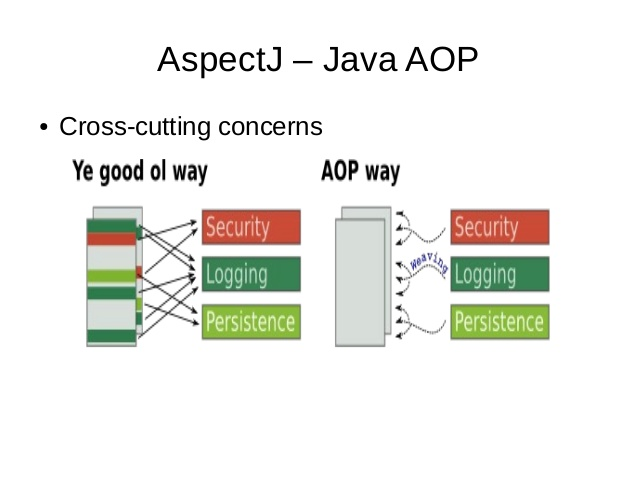
\includegraphics[width=1\textwidth]{images/aspect.jpg}
	\caption{Cross Cutting Concerns in AspectJ (Abbildung aus \cite{asp})}
	\label{fig:aop}
\end{figure}

\newpage
\paragraph{TranSAT Struktur}
TranSAT (Transform Software Architecture Technologies) ist ein Framework, welches es erm�glicht, bestehende Softwarearchitekturmodelle um neue Concerns zu erweitern. Dabei l�sst TranSAT nur konsistente Ver�nderungen zu.\\
Daf�r besitzt TranSAT  ein Basissoftwarearchitekturmodel bzw. auch Softwarearchitekturspezifikation genannt, welches die bisherige Architektur beschreibt. Dieses kann dann mit den Prinzipien der Aspekt Orientierte Programmierung durch neue Concerns erweitert werden. Typische Concerns sind persistence, security oder Transaktionsmanagement.\\
\cite{SAE},\cite{TranSAT}\\
\subparagraph{Concerns:}
Daf�r m�ssen die Concerns unabh�ngig von dem bestehenden Basissoftwarearchitekturmodel bzw. des Kontextes spezifiziert werden. Dies erm�glicht zudem noch eine leichtere Wiederverwendung der Concerns.\\
H�ufig sind diese neuen Concerns Cross-Cutting-Concerns, alse sie ver�ndern mehrere Gesch�ftslogikkomponenten, sowie das Interaktionsverhalten zwischen verschiedene Komponenten.\\
Daf�r m�ssen dann die Integrationsregeln spezifiziert werden.\\
Damit TranSAT aus dem Basissoftwarearchitekturmodel und dem Concern ein neues Softwarearchitekturmodell erstellen kann, werden wie in \ref{fig:TranSAT} zu sehen die Konzepte des Adapters und des Weavers verwendet.\\
\cite{TranSAT}\\
\subparagraph{Adapter:}
Im Adapter sind wie in \ref{fig:TranSAT2} zu sehen, die Integrationsregeln spezifiziert. Der Adapter kennt den Kontext nicht, besitzt jedoch wie in \ref{fig:TranSAT2} zu sehen eine Point-Cut-Mask. Die Point-Cut-Mask eine Art Vertrag, welcher definiert, wie die Umgebung auszusehen hat, damit der Concern richtig in die Architektur integriert werden kann.\\
\cite{TranSAT}\\
\subparagraph{Weaver:}
Der Weaver vergleicht die Informationen aus dem Adapter mit denen des bestehenden Basisarchitekturmodels. Dabei vergleicht er die Point-Cut-Mask des Concerns mit der Point-Cut-Definition im Basisarchitekturmodel und pr�ft ob die Integrationsregeln angewandt werden k�nnen. Dann f�gt er den neuen Concern gem��t der Integrationsregeln an den Stellen in das Basisarchitekturmodell an denen die Point-Cut-Mask und  die Point-Cut-Definition �bereinstimmen ein und erzeugt so ein neues Architekturmodell\ref{fig:TranSAT}.\\
\cite{TranSAT}\\

 \begin{figure}
	\centering
	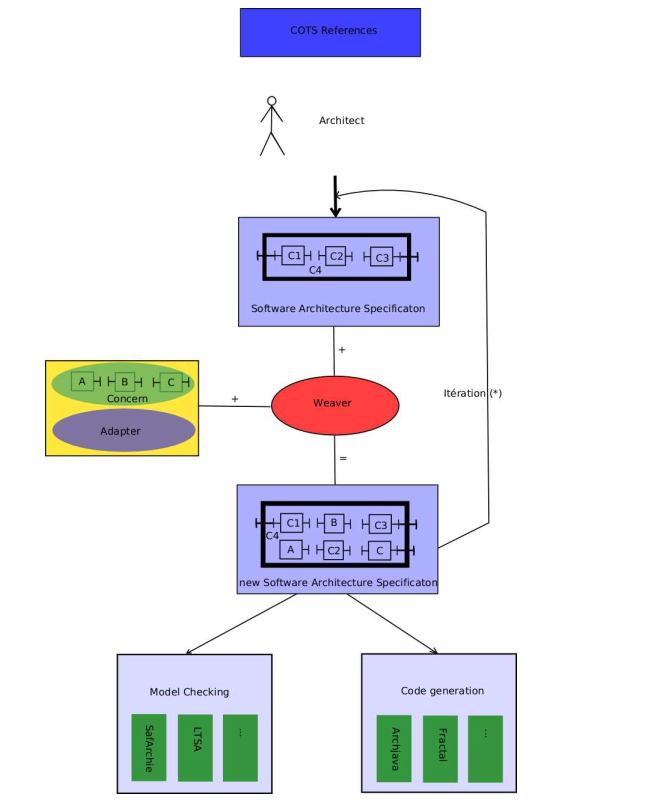
\includegraphics[width=1\textwidth]{images/TranSAT.png}
	\caption{TranSat �bersicht (Abbildung aus \cite{TranSAT}, S.4)}
	\label{fig:TranSAT}
\end{figure}


 \begin{figure}
	\centering
	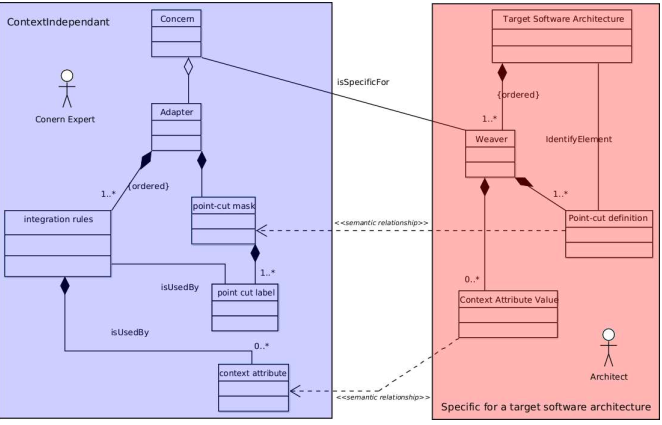
\includegraphics[width=1\textwidth]{images/TranSAT2.png}
	\caption{TranSat meta-model (Abbildung aus \cite{TranSAT}, S.5)}
	\label{fig:TranSAT2}
\end{figure}
%\paragraph{TranSat Demo: Bankanwendung}

%\subparagraph{Erweiterung um Atomarit�ts Concern}

\newpage
%%________________________________________________________________
\section{Undokumentierte Architekturen}
In vielen Softwareprojekten gibt es keine Architekturdokumentationen. Auff�llig ist, das viele OpenSource-Projekte die Architektur nicht dokumentieren.(\cite{Role}S.246)\\
Dies verst��t gegen den Concern Erhaltung von Wissen \ref{Wissen}.

\paragraph{Ursachen}
M�gliche Ursachen k�nnten wohl sein, dass sich keine Gedanken �ber die Architektur gemacht wurden und \glqq einfach drauf los programmiert wird \grqq oder dass wenn sich Gedanken gemacht wurden diese nicht dokumentiert werden, da die geplante Architektur im Team als \glqq selbsverst�ndlich\grqq selbstverst�ndlich gilt. (Habe beides in verschiedenen Projekten miterlebt.)
  
\paragraph{Folgen}
Im Laufe der Zeit geht das Wissen �ber die Architektur verloren, falls es �berhaupt vorhanden war. Daraus resultiert dann dass das Projekt im Laufe der Zeit komplexer wird, ohne dass eine �bersicht �ber die Architektur existiert und die Software somit schlecht zu warten oder erweitern ist.

\paragraph{Folgenreduktion}
Im laufe der Zeit wurden Verschiedene Techniken zum Reverseengineering der Architektur erarbeitet.\cite{Role}
Beispiele daf�r w�ren: Package View, Bunch View \cite{otam}, ArchDRH View \cite{ldrt}oder ACDC View \cite{acdc}.\\
Sobald dies gemacht wurde, kann mit diese dann analysiert, evaluiert und verbessert werden.

%%________________________________________________________________
\section{Nicht Gewartete Architekturen/Architekturmodell Anders Als Implementierung}
Viele Projekte besitzen zwar eine Architekturdokumentation, diese ist jedoch h�ufig nicht vertrauensw�rdig.(\cite{Role}, S.249)
\paragraph{Ursachen}
Viele Ans�tze f�r ADLs entkoppeln den implementierten Code von der Architekturbeschreibung.(\cite{Role}, S.4)

\paragraph{Folgen}
Es kann dazu kommen, dass die Architekturbeschreibung nicht mit dem eigentlichen Code �bereinstimmt und somit inkonsistent ist. Der Code kann dadurch geplante Architektureigenschaften verletzen. Und es wird un�bersichtlich, wenn Code und Architekturbeschreibung nicht �bereinstimmen.
Auch hier liegt ein Versto� gegen den Concern Erhaltung von Wissen \ref{Wissen} vor.

\paragraph{Risikoreduktion}
Es ist hilfreich ADLs zu verwenden, welche eng mit dem Code gekoppelt sind. Beispiele daf�r w�ren ArchJava, Fractal oder Sofa.(\cite{Role}, S.4)

\paragraph{Folgenreduktion}
Sollte es sich eingeschlichen haben, dass das Architekturmodell anders ist als die Implementierung, kann genauso vorgegangen werden, wie wenn keine Dokumentation vorliegt. Evtl. kann es hier sinnvoll sein, das soll-modell und das ist-Modell zu vergleichen.

%%________________________________________________________________
\section{Priorisierung der Falschen Dimensionen}

\paragraph{Ursachen}
Bei der Festlegung f�r die Unterst�tzung �nderungsm�glichkeiten kann es vorkommen, dass die Dimensionen st�rker ber�cksichtigt werden, die einem bekannt sind.\\
Es ist auch m�glich, dass bestimmte Dimensionen wichtiger erscheinen, als sie sind, da  lautstarke Stakeholder diese besonders h�ufig erw�hnen.

\paragraph{Folgen}
Die Software wird zu komplex und zu teuer. Au�erdem ist es m�glich, dass sollten �nderungen in anderen Dimensionen vonn�ten sein, diese sogar schwieriger werden als wenn die Software mit einer einfacheren Architektur implementiert worden w�re.

\paragraph{Risikoreduktion}
Es sollte nur nach ausreichender Analyse entsprechende Unterst�tzung f�r die �nderungen eingebaut werden, um diese richtig zu priorisieren.\\
(\cite{SSA:12}, S.560)


%%________________________________________________________________
\section{�nderungen die nie kommen}
Es ist schlichtweg unm�glich, eine Softwarearchitektur mit vertretbaren Kosten und Risiken zu entwickeln, welche alle m�glichen �nderungen unterst�tzt.(\cite{SSA:12}S.561)
\paragraph{Ursachen}
Bei der Entscheidung, welche Arten von �nderungen unterst�tzt werden, wurde falsch entschieden.
\paragraph{Folgen}
Die Unterst�tzung von �nderungen verursacht Overhead im Design, in der Implementierung und h�ufig auch zur Laufzeit. Daher verursacht es unn�tige Kosten, wenn die �nderungen die unterst�tzt werden, nie kommen.
\paragraph{Risikoreduktion}
Die Bereitstellung der Unterst�tzung bestimmter Arten von �nderungen durch die Architektur sollte nur mit ausreichender Sicherheit, dass diese auch eintreten.
\paragraph{Folgenreduktion}
Sollte auffallen, dass �nderungen, f�r die schon eine eingebaute Unterst�tzung vorhanden ist, nie kommen, so sollte diese Unterst�tzung als Ballast betrachtet  und dementsprechend entfernt werden. \\
(\cite{SSA:12}, S.561)
%%________________________________________________________________
\section{Auswirkungen auf andere kritische Qualit�tseigenschaften}

\paragraph{Ursachen}
Meistens sind hochflexible Systeme unperformant, besitzen eine hohe Komplexit�t und sind dementsprechend teuer in der Entwicklung.
\paragraph{Folgen/Gefahren}
Daher steht die Fokussierung auf Flexibilit�t h�ufig im direkten Widerspruch zu anderen Qualit�tseigenschaften, wie z.B. die Performanz oder die Benutzbarkeit.\\
Zus�tzlich kommt es vor, dass durch die zu starke Fokussierung auf die Flexibilit�t durch Zeitdruck andere Qualit�tseigenschaften vernachl�ssigt werden.

\paragraph{Risikoreduktion}
Es muss f�r ein Projekt eine passende Balance zwischen den verschiedenen Qualit�tseigenschaften gefunden werden. Daf�r ist ein Prozess der kontinuierlichen Beurteilung der Architektur hilfreich.\\
(\cite{SSA:12}, S.561-562)

%%________________________________________________________________
\section{Zu Starke Abh�ngigkeit von spezifischer Hard- oder Software}


\paragraph{Vorteile}
Fremde Soft-/Hardware zu verwenden kann ggf. preiswerter sein als alles selbst zu entwickeln.
Zudem sind dadurch k�rzere Entwicklungszeiten m�glich.
\paragraph{Nachteile/Gefahren}
Es kann sein, dass die verwendeten Komponenten nicht mehr verf�gbar sind. Bei Hardware k�nnte es sein, dass diese kaputt geht und evtl. nicht mehr hergestellt werden und bei Software z.B. dass Vertr�ge auslaufen.\\
Es kann auch sein, dass irgendwann bestimmte Komponenten theoretisch  durch bessere oder preiswertere Komponenten ausgetauscht werden k�nnten, jedoch die eigene Software speziell auf die eine Komponente angepasst ist und somit diese Komponente faktisch nicht austauschbar ist.
\paragraph{Risikoreduktion}
\subparagraph{1.}
Vor der Verwendung von spezifischer Hard- oder Software sollte vorher abgewogen werden, ob die Vorteile �berwiegen.
\subparagraph{2.}
Sollte entschieden worden sein, dass die Vorteile �berwiegen, gilt es die Roadmaps der Verk�ufer, so wie die anderen Faktoren die das Leben der Komponenten beeinflussen, zu ber�cksichtigen. Also z.B. lieber zus�tzliche Hardware zu kaufen, die als Ausfallersatz dient, sollte verwendete Hardware kaputt gehen.
\subparagraph{3.}
Die Auswirkungen durch �nderungen der spezifischen Komponenten sollte durch eine entsprechende Abstraktion der der Schnittstellen zu diesen erfolgen.
(\cite{SSA:12}, S.562)
%%________________________________________________________________
\section{Verlorengegangene Entwicklungsumgebung}

\paragraph{Ursachen}
Die Entwicklungs- und Testumgebungen gehen leichter verloren, als die Deploymentumgebung.
Zus�tzlich unterliegen Entwicklungsumgebungen einer von der Deploymentumgebung unabh�ngigen Evolution, da sich Entwicklungs- und Supportpriorit�ten sowie Arbeitspensum  sich �ber Zeit �ndern.

\paragraph{Folgen/Gefahren}
Soll nun ein bestimmter Stand einer Entwicklungs- oder Testumgebungen wiederhergestellt werden, fehlt h�ufig dass Wissen dar�ber, was alles ben�tigt wird und was zu tun ist.

\paragraph{Ben�tigtes Wissen bei der Wiederherstellung}
Um eine entsprechende Entwicklungsumgebung wiederherzustellen, m�ssen folgende Fragen beantwortet werden k�nnen.\\
Wird eine spezielle Version einer Library ben�tigt? Oder funktioniert eine neuere Version auch?\\
Welche Werkzeuge (mit welchen Versionen?) werden f�r den kompletten Build- und Releaseprozess ben�tigt?
Sind spezielle Skripte im Einsatz? Werden daf�r irgendwelche Erweiterungen ben�tigt?\\
Ben�tigen die verwendeten Entwicklungswerkzeuge spezielle Patches? \\
Wird eine bestimmte OS-Version ben�tigt? Oder ein bestimmtes Modell von Hardwarekomponenten? Oder sind diese durch neuere Versionen ersetzbar?\\

\paragraph{Risikoreduktion}
Zun�chst sollte der Name, die Version, der Ursprung und der Grund f�r die Einf�hrung, bei der Einf�hrung externer Elemente in die Entwicklungsumgebung dokumentiert werden. Als informelles Textdatei innerhalb des verwendeten Konfigurationsmanagementsystems sollte ausreichen.\\
Um zu vermeiden, dass die so gesammelten Informationen unvollst�ndig sind, sollte am Ende der Konstruktionsphase die Entwicklungsumgebung woanders nur mit den gesammelten Informationen erneut aufgesetzt und getestet werden. Dabei f�llt auf, ob noch was vergessen wurde. Sollte dabei auffallen, dass was vergessen wurde sollte dies mit aufgenommen werden und dann erneut aufgesetzt und getestet werden, so wird erspart, dass die L�cken erst auffallen, wenn das Wissen dar�ber bereits vergessen wurde.\\
Wenn m�glich ist es sinnvoll, Hardware Virtualisierungstechniken zu verwenden, um die Umgebung zu erhalten.\\
Sollten kritische oder nur schwer zu beschaffende Hardwarekomponenten verwendet werden, ist es au�erdem noch sinnvoll von denen Ersatzteile zu besitzen.\\
(\cite{SSA:12}, S.562-563)

%%________________________________________________________________
\section{Ad	Hoc Release Management}
Das Deployen in eine Testumgebung birgt normalerweise kein Risiko. Sollten dabei Fehler auftreten, so k�nnen diese in Ruhe behoben und dann nochmals deployt werden, ohne dass Benutzer betroffen sind.\\
Wenn jedoch Fehler beim Deployen in eine Produktivumgebung entstehen, k�nnen diese von nervig f�r Benutzer und Admins bis hin zu einer Gef�hrdung der kritischen Operationen der Zielorganisation werden.
Daher wird ein Releasemanagement ben�tigt.

\paragraph{Risikoreduktion}
\label{release}
Der Release-Prozess sollte soweit wie m�glich automatisiert werden. Dies erh�ht die Zuverl�ssigkeit und Wiederholbarkeit. Sobald der Release-Prozess einmal automatisiert wurde, sinkt der Aufwand bei weiteren Releases. Zus�tzlich verringert dies die menschlichen Fehler, die w�hrend des Release-Prozess auftreten.




% ...
%--------------------------------------------------------------------------
\backmatter                        		% Anhang
%-------------------------------------------------------------------------
\bibliographystyle{geralpha}			% Literaturverzeichnis
\bibliography{literatur}     			% BibTeX-File literatur.bib
%--------------------------------------------------------------------------
\printindex 							% Index (optional)
%--------------------------------------------------------------------------
\begin{appendix}						% Anh�nge sind i.d.R. optional
   \chapter{Glossar}

\abbreviation{DisASTer}		{DisASTer (Distributed Algorithms Simulation Terrain), A platform for the Implementation of Distributed Algorithms}
\abbreviation{DSM}			{Distributed Shared Memory}
\abbreviation{AC}			{Linearisierbarkeit (atomic consistency)}
\abbreviation{SC}			{Sequentielle Konsistenz (sequential consistency)}
\abbreviation{WC}			{Schwache Konsistenz (weak consistency)}
\abbreviation{RC}			{Freigabekonsistenz (release consistency)}
			% Glossar   
\end{appendix}

\end{document}
